\documentclass[../Head/report.tex]{subfiles}
\begin{document}

\definecolor{codegreen}{rgb}{0,1.0,1.0}
\definecolor{codegray}{rgb}{0.5,0.5,0.5}
\definecolor{codepurple}{rgb}{1.0,1.0,0.6}
\definecolor{backcolour}{rgb}{0.92,0.92,0.92}

\lstdefinestyle{mystyle}{
    backgroundcolor=\color{backcolour},   
    commentstyle=\color{codegreen},
    keywordstyle=\color{magenta},
    numberstyle=\tiny\color{codegray},
    stringstyle=\color{codepurple},
    basicstyle=\footnotesize,
    breakatwhitespace=false,         
    breaklines=true,                 
    captionpos=b,                    
    keepspaces=true,                 
    numbers=left,                    
    numbersep=5pt,                  
    showspaces=false,                
    showstringspaces=false,
    showtabs=false,                  
    tabsize=2
}

\lstset{style=mystyle}

\section{Materials}
This section deals with the materials used to build the UAV, for communication and onboard computing. A description of the different products and a wiring diagram for the UAV platform will be analyzed in Section \ref{sec:hardware}. In Section \ref{sec:bill_of_materials}, the bill of materials is discussed with the overall cost of the implementation in regard to hardware.   

\subsection{Hardware}
\label{sec:hardware}

The UAV used is a Holybro Pixhawk 4 mini QAV250 Quadcopter. The reason for choosing this kit is because of the Pixhawk 4 mini which is part of the product. PX4 is open source and has a lot of features together with a discussion forum for debugging and knowledge sharing of the general system. The software part of PX4 will be discussed in Section \ref{sec:px4_flight_stack}. The UAV can be seen in Figure \ref{fig:holybro_pixhawk_mini_drone}. 

For communication between the pilot and UAV, a FlySky FS i6 transmitter is used. Though this is a basic transmitter it offers great features together with a receiver for a low price. The transmitter and receiver can be seen in Figure \ref{fig:flysky_transmitter}. 

\begin{figure}[H]
    \centering
    \begin{subfigure}[b]{.4\textwidth}
        \centering
        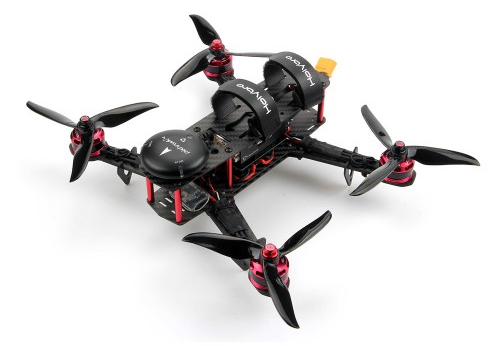
\includegraphics[height=4.0cm]{../Figures/drone/holybro_pixhawk_mini.png}
           %\vspace{0.5em}
        \caption{}
        \label{fig:holybro_pixhawk_mini_drone}
    \end{subfigure}
    %\hspace{-2.8em}
    \begin{subfigure}[b]{.33\textwidth}
        \centering
        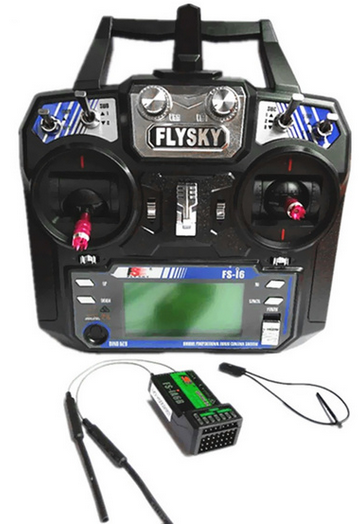
\includegraphics[height=4.0cm]{../Figures/drone/flysky_transmitter.png}
        \caption{}
        \label{fig:flysky_transmitter}
    \end{subfigure}
    \caption{Illustration of the \href{https://www.banggood.com/da/Holybro-Pixhawk-4-Mini-QAV250-Basic-Kit-RC-Quadcopter-RC-Drone-W-or-Pixhawk-4-GPS-DR2205-KV2300-Motor-p-1438132.html?utm\_source=googleshopping&utm\_medium=cpc\_organic&gmcCountry=DK&utm\_content=minha&utm\_campaign=minha-dk-da-pc&currency=DKK&cur\_warehouse=CN&createTmp=1&ID=567322&utm\_source=googleshopping&utm\_medium=cpc\_union&utm\_content=sandra&utm\_campaign=sandra-ssc-dk-da-all-0302&ad\_id=337427030565&gclid=CjwKCAjwmv-DBhAMEiwA7xYrd4Bgzi1gPmtia01iAeXnLyVW9CXudMOZ7eQxM53PrTrgx2OHdLvS1hoCdPIQAvD\_BwE}{Holybro Pixhawk 4 Mini QAV250} UAV in Figure \ref{fig:holybro_pixhawk_mini_drone} and \href{https://www.banggood.com/FlySky-FS-i6-2\_4G-6CH-AFHDS-Remote-Control-Transmitter-With-FS-R6B-Receiver-For-RC-FPV-Drone-Mode-2-p-1420323.html?utm\_source=googleshopping&utm\_medium=cpc\_organic&gmcCountry=DK&utm\_content=minha&utm\_campaign=minha-dk-en-pc&currency=DKK&cur\_warehouse=CN&createTmp=1&utm\_source=googleshopping&utm\_medium=cpc\_bgs&utm\_content=sandra&utm\_campaign=sandra-ssc-dk-en-all-1105-20bf-11sale&ad\_id=477449337289&gclid=CjwKCAjwmv-DBhAMEiwA7xYrdwTH-q0\_ud-CLZ7CMggdiHnZUga0M4Bhc-nwwN5mUIZsSw1DH_ltyxoCsdoQAvD\_BwE}{flysky transmitter} in Figure \ref{fig:flysky_transmitter}}
    \label{fig:holybro_pixhawk_mini}
\end{figure}

Because the UAV and onboard computer has to be powered separately, two gens ace LiPo batteries with 11.1V and 2200 mAh have been considered. These batteries matches the XT60 connection which is used by the power board of the kit. The reason for choosing these as 3-cell batteries compared to 4-cell, is to reduce the height of center of mass of the UAV which could make the system unstable because the batteries are placed above the propellers as seen in Figure \ref{fig:holybro_pixhawk_mini_drone}. The UAV and Raspberry Pi has to be powered separately because the Raspberry Pi has to be given constant 5 volts and 3 amps for best performance. If the Raspberry Pi is giving under- or over-voltage, the Pi could potentially shut down which could be fatal if the UAV where relying on pose estimates from the onboard computer. The used LiPo battery can be seen in Figure \ref{fig:gens_ace_lipo_battery}.  

\begin{figure}[H]
    \centering
    \hspace{-1.0em}
    \begin{subfigure}[b]{.25\textwidth}
        \centering
        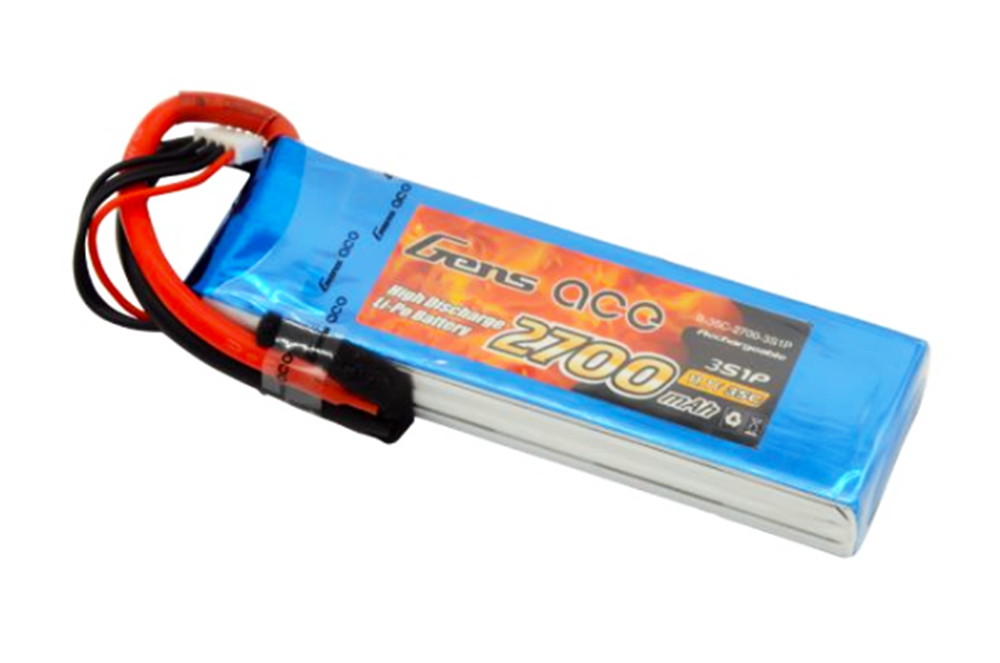
\includegraphics[height=2.0cm]{../Figures/batteries/lipo_one.png}
        \caption{}
        \label{fig:gens_ace_lipo_battery}
    \end{subfigure}
    %\hspace{-2.8em}
    \begin{subfigure}[b]{.20\textwidth}
        \centering
        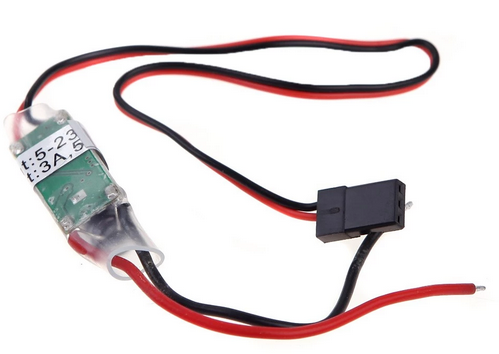
\includegraphics[height=2.0cm]{../Figures/batteries/ubec_3A_power_converter.png}
        \caption{}
        \label{fig:ubec_3A_power_converter}
    \end{subfigure}
        \begin{subfigure}[b]{.20\textwidth}
        \centering
        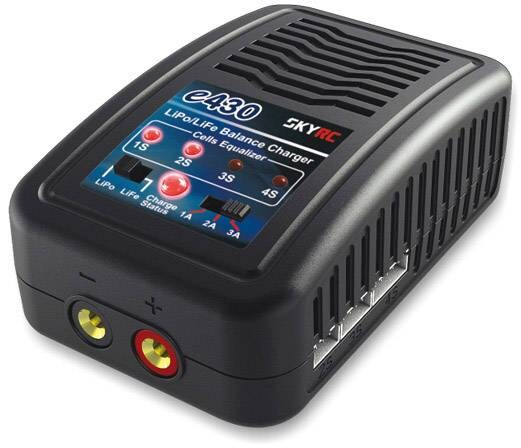
\includegraphics[height=2.0cm]{../Figures/batteries/balance_charger_sky_rc.jpg}
        \caption{}
        \label{fig:balance_charger_sky_rc}
    \end{subfigure}
            \begin{subfigure}[b]{.25\textwidth}
        \centering
        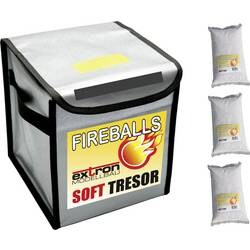
\includegraphics[height=2cm]{../Figures/batteries/lipo_battery_case.jpg}
        \caption{}
        \label{fig:lipo_battery_case}
    \end{subfigure}
    \caption{The used materials for battery and power configurations. The used \href{https://www.conradelektronik.dk/p/gens-ace-modelbyggeri-batteripakke-lipo-111-v-2200-mah-celletal-3-45-c-xt60-2145181?gclid=CjwKCAjwmv-DBhAMEiwA7xYrdyX00RZAovYbKhjWqit3MYObx_NtIH_NOxPih2MBqFoyuJrHtL_R7xoCg28QAvD_BwE&gclsrc=aw.ds&utm_campaign=shopping-feed&utm_content=free-google-shopping-clicks&utm_medium=surfaces&utm_source=google&utm_term=2145181&vat=true}{Gens ace LiPo battery} in Figure \ref{fig:gens_ace_lipo_battery}, \\ \href{https://hobbyking.com/en_us/kingkong-5v-3a-ubec.html?___store=en_us}{Ubec 3A power converter} in Figure \ref{fig:ubec_3A_power_converter}, \href{https://www.banggood.com/da/SKYRC-E430-Balance-Charger-AC-100-240V-Cells-Lipo-LiFe-30W-1A-2A-3A-p-1124821.html?utm_source=googleshopping&utm_medium=cpc_organic&gmcCountry=DK&utm_content=minha&utm_campaign=minha-dk-da-pc&currency=DKK&cur_warehouse=CN&createTmp=1&utm_source=googleshopping&utm_medium=cpc_union&utm_content=sandra&utm_campaign=sandra-ssc-dk-da-all-0302&ad_id=337427030565&gclid=CjwKCAjwmv-DBhAMEiwA7xYrdwCnJMgzOnZp9FJBPNSDSS_RO2Q67TIQ2FderUjGhzySiWRObpBN6xoCtE4QAvD_BwE}{SKYRC balance charger} in Figure \ref{fig:balance_charger_sky_rc} and \href{https://cdon.dk/hjem-have/extron-modellbau-lipo-safety-bag-1-set-p47436624?fo_c=1923&fo_k=47efd6de4697e54ef539b8256db201cb&fo_s=gpladk&utm_medium=cpo&utm_source=tradedoubler&utm_campaign=affiliate&utm_content=tradedoubler_3153538_General_VelkashoppingcomDK}{LiPo safety-bag} in Figure \ref{fig:lipo_battery_case}}
    \label{fig:battery_and_power_connections}
\end{figure}

To convert the input voltage from the LiPo battery to the Raspberry Pi, a KINGKONG 5V 3A Switching Power UBEC converter for switching between 7.4-22.2V (2-6S LiPoly) to constant 5V/3A is used. The setup of this requires a little soldering where the ends of the wires have to be soldered to a XT60 connector to be used to connect to the LiPo battery, where the output of this is connected to the 5V and ground pins of the raspberry Pi. This switch can be seen in Figure \ref{fig:ubec_3A_power_converter}. 

To charge the LiPo batteries, a SKYRC balance charger is used. This unit can charge 2-4 cell batteries with constant 1-3 amps of current which fits the 2200 mAh batteries. Moreover, it includes a XT60 charging cable which matches the already mentioned connectors. This charger can be seen in Figure \ref{fig:balance_charger_sky_rc}.

Because LiPo batteries can be dangerous and may cause fire if damaged or overcharged \cite{lipoBatteryGuide}, a LiPo safety bag is used as seen in Figure \ref{fig:lipo_battery_case}. This bag includes \textit{fireballs} which encapsulates the possible fire of the batteries to be only in the safety bag. 

In order to achieve serial communication between the PX4 and the Raspberry Pi, the universal asynchronous receiver-transmitter (UART) port of the PX4 is used via a 6 pin connection cable seen in Figure \ref{fig:six_pin_serial_connection_cable}. Either two ways could be used to achieve serial communication from the point of view of the Raspberry Pi. One method is to use the general purpose input output (GPIO) pins of the Pi which is Tx (transmit) and Rx (receive). If choosing this setup, the data will be transmitted through the \textit{/dev/ttyS0} port of the Raspberry Pi where you got to have read/write privileges or being part of the group \textit{tty} to do so. These settings can be changed accordingly from the terminal in Ubuntu as seen in Listing \ref{lst:change_permissions}. 

\definecolor{lightgreen}{rgb}{0.56, 0.93, 0.56}
\definecolor{moonstoneblue}{rgb}{0.45, 0.66, 0.76}
\begin{listing}[H] 
\begin{tcolorbox}[
    enhanced,
    attach boxed title to top left={xshift=6mm,yshift=-3mm},
    colback=lightgreen!20,
    colframe=lightgreen,
    fonttitle=\bfseries\color{black},
]
\begin{minted}[ numbersep=6pt, linenos=true, breaklines=true, breakanywhere=true, mathescape, escapeinside=||,fontsize=\small]{bash}
$ cd chmod a+rw /dev/ttyS0
$ usermod -a -G tty ubuntu
\end{minted}
\end{tcolorbox}
\caption{How to change read/write permissions along with adding a user (ubuntu) to the tty group}
\label{lst:change_permissions}    
\end{listing} 

The other method is to connect the 6 pin connection cable to a TTL 232R cable seen in Figure \ref{fig:usb-TTL_232R_Raspberry_Pi_debug} to the universal serial bus (USB) port of the Raspberry Pi. This can easily be done by solder the Tx, Rx and ground parts of the two cables together. Some benefits comes by using the later solution e.g no problems with u-boot of the Raspberry Pi when the PX4 transmit data on the GPIO pins during boot up of the system  \cite{uBoot}. The latter option is used.

\begin{figure}[H]
    \centering
    \hspace{-4.0em}
    \begin{subfigure}[b]{.3\textwidth}
        \centering
        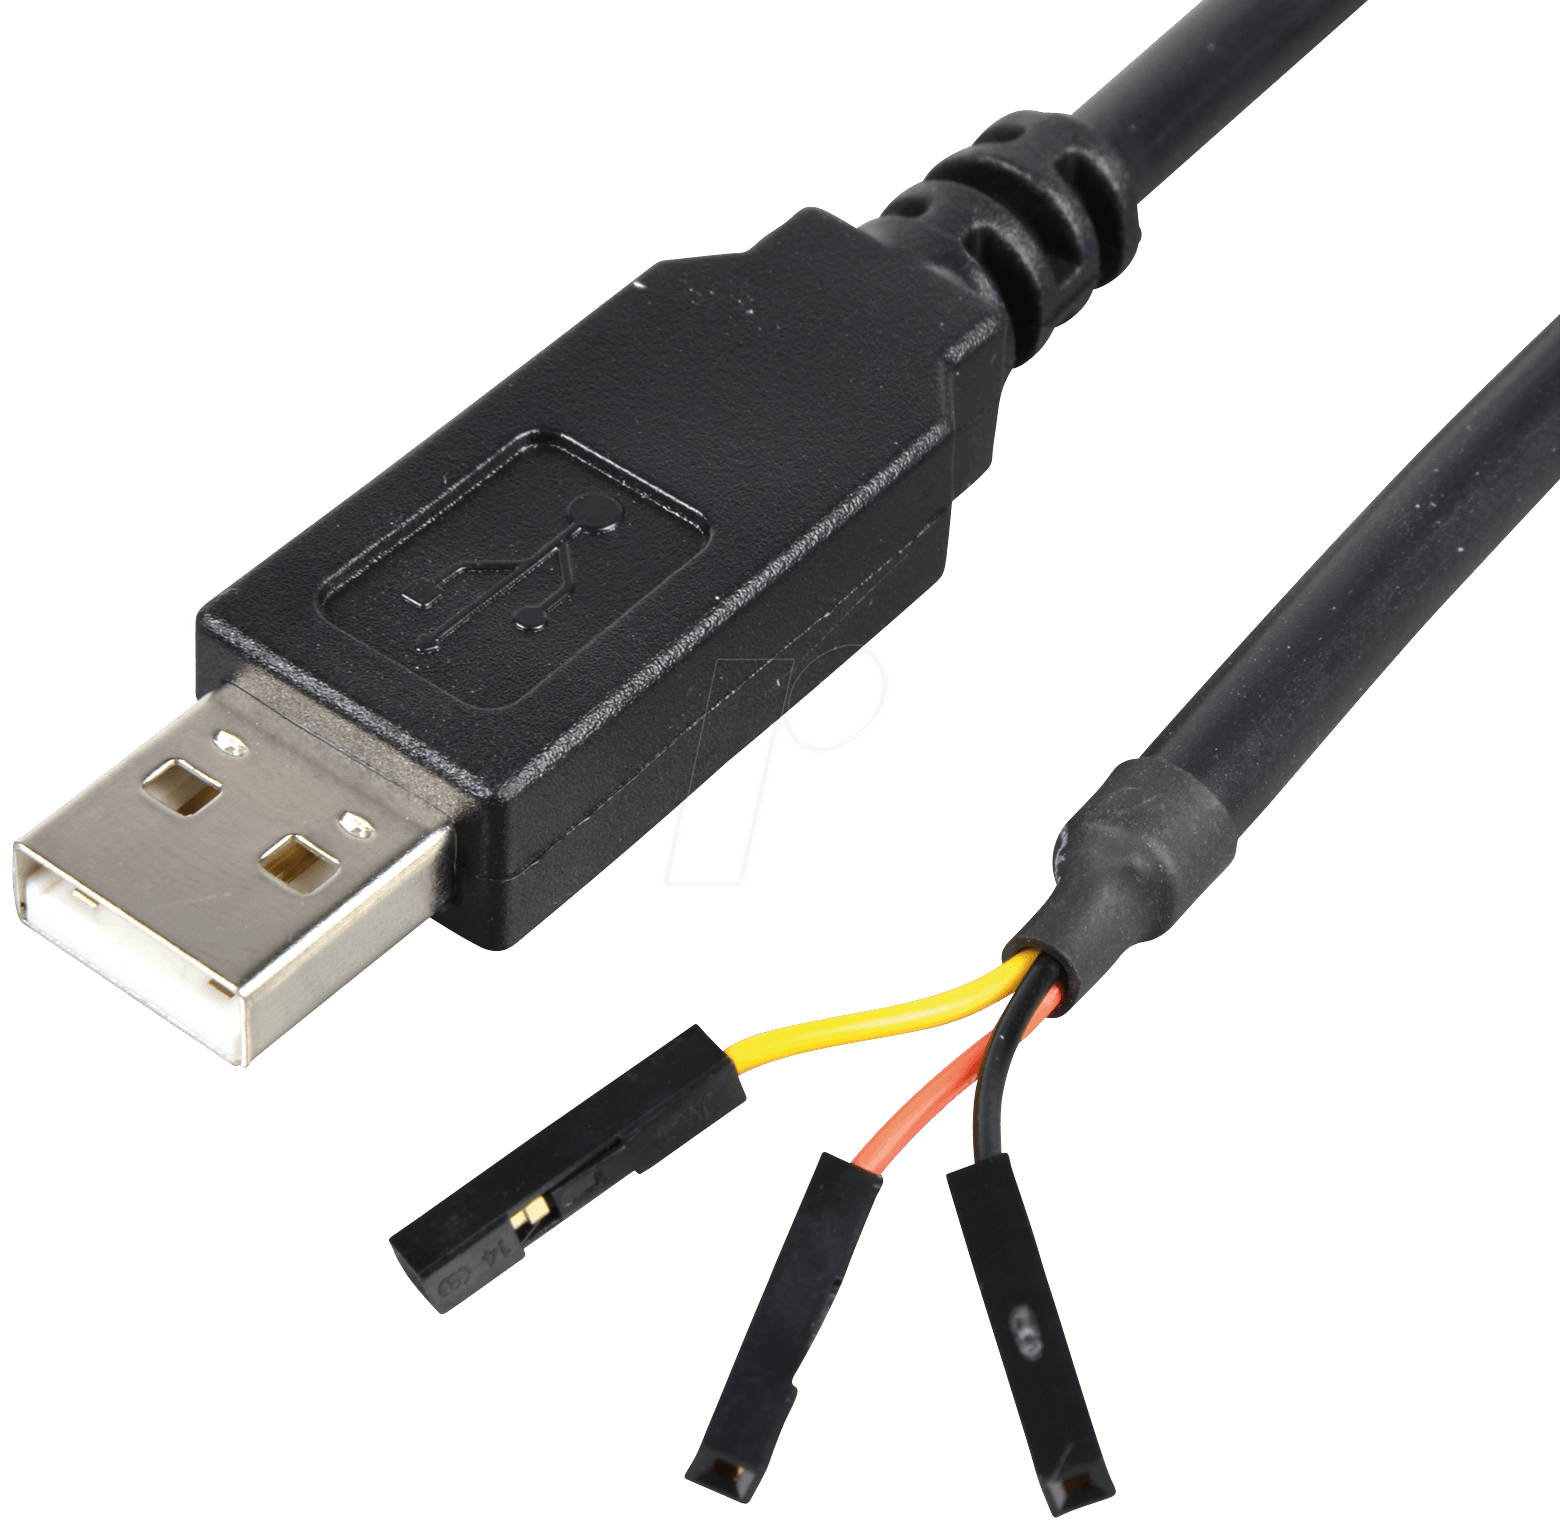
\includegraphics[height=3cm]{../Figures/raspberry_pi/usb-TTL_232R_Raspberry_Pi_debug.png}
        \caption{}
        \label{fig:usb-TTL_232R_Raspberry_Pi_debug}
    \end{subfigure}
    %\hspace{-2.8em}
    \begin{subfigure}[b]{.25\textwidth}
        \centering
        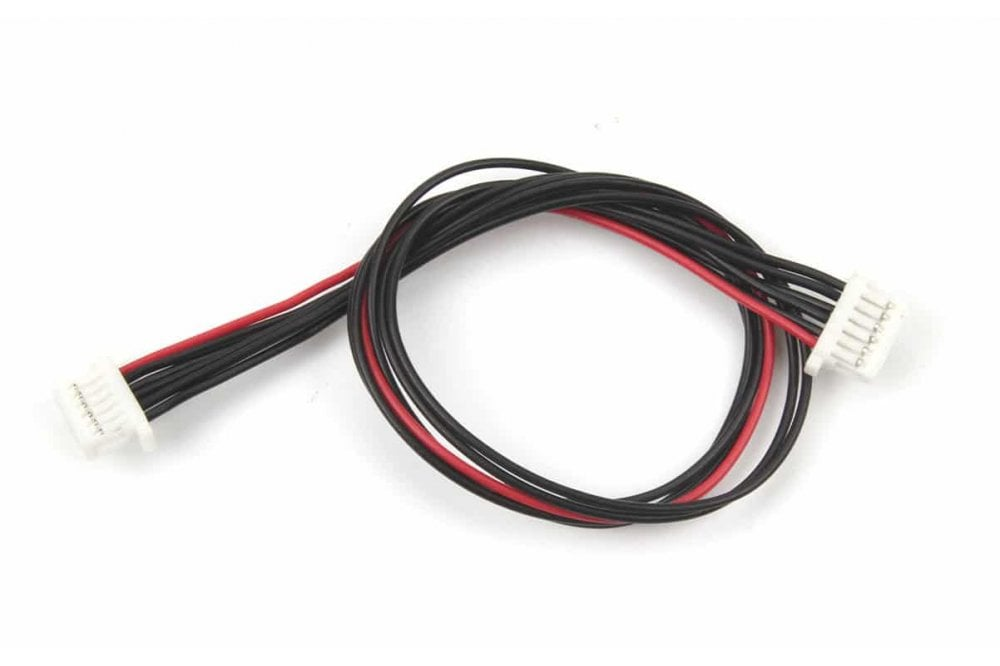
\includegraphics[height=3cm]{../Figures/raspberry_pi/holybro-pixhawk-4-mini-uart-cable.jpg}
        \caption{}
        \label{fig:six_pin_serial_connection_cable}
    \end{subfigure}
    \caption{Cables for serial communication between the PX4 flight conrtoller and raspberry Pi. To enable the use of serial communication from the USB of the raspberry Pi, a \href{https://raspberrypi.dk/en/product/usb-to-ttl-rs232-debug-cable-for-raspberry-pi/}{USB to TTL-RS232} cable is used which can be seen in Figure \ref{fig:usb-TTL_232R_Raspberry_Pi_debug} and a six pin serial connection cable in Figure \ref{fig:six_pin_serial_connection_cable}}
    \label{fig:pixhawk_mini_four}
\end{figure}

In regard to the onboard computer, a Raspberry Pi 4B with 8 GB of random access memory (RAM) is seen in Figure \ref{fig:raspberry_pi}. Other onboard computers like Jetson Nano was also considered. However, because of the price, size, computational capabilities and large community of knowledge sharing the Raspberry Pi is used. Here the operation system Ubuntu 18.04.5 LTS (Bionic Beaver) 64-bit server edition will be implemented. This is further discussed in Section \ref{sec:companion_computer}.

Because the central processing unit (CPU) of the Raspberry Pi can overheat during constant computational load, a fan is used to cool down the Raspberry Pi during operation. The Shim fan along with the fan attached to the Raspberry Pi can be seen in Figures \ref{fig:raspberry_pi_shim_fan} and \ref{fig:raspberry_pi} respectively. Moreover, by using active cooling instead of passive cooling e.g a aluminum heat-sink Case, the weight of the Pi is reduced. This also enables the use of overclocking of the Raspberry Pi for better performance which is discussed in Section \ref{sec:companion_computer}.

To safely attache the Raspberry Pi on to the UAV, a transparent case is used as seen in Figure \ref{fig:raspberry_pi_case}. This case is appropriate because it can store both the Shim fan and Raspberry Pi camera without any chance of damage to the hardware on the board. In order to control the UAV using WiFi, a WiFi adapter seen in Figure \ref{fig:tpLinkac} is used in order to get ground truth data from the Optitrack system. This is discussed in Section \ref{sec:companion_computer} and \ref{sec:optitrack_system}.

A Logitech C270 HD camera is used as the front camera and a Raspberry Pi V2 as bottom camera as seen in Figures \ref{fig:raspberry_pi_front_cam} and \ref{fig:raspberry_pi_bottom_cam} respectively. The Logitech camera will be attached to the USB port of the Raspberry Pi while the Raspberry Pi camera is connected through the camera serial interface (CSI). 

\begin{figure}[H]
    \centering
    \begin{subfigure}[b]{.13\textwidth}
        \centering
        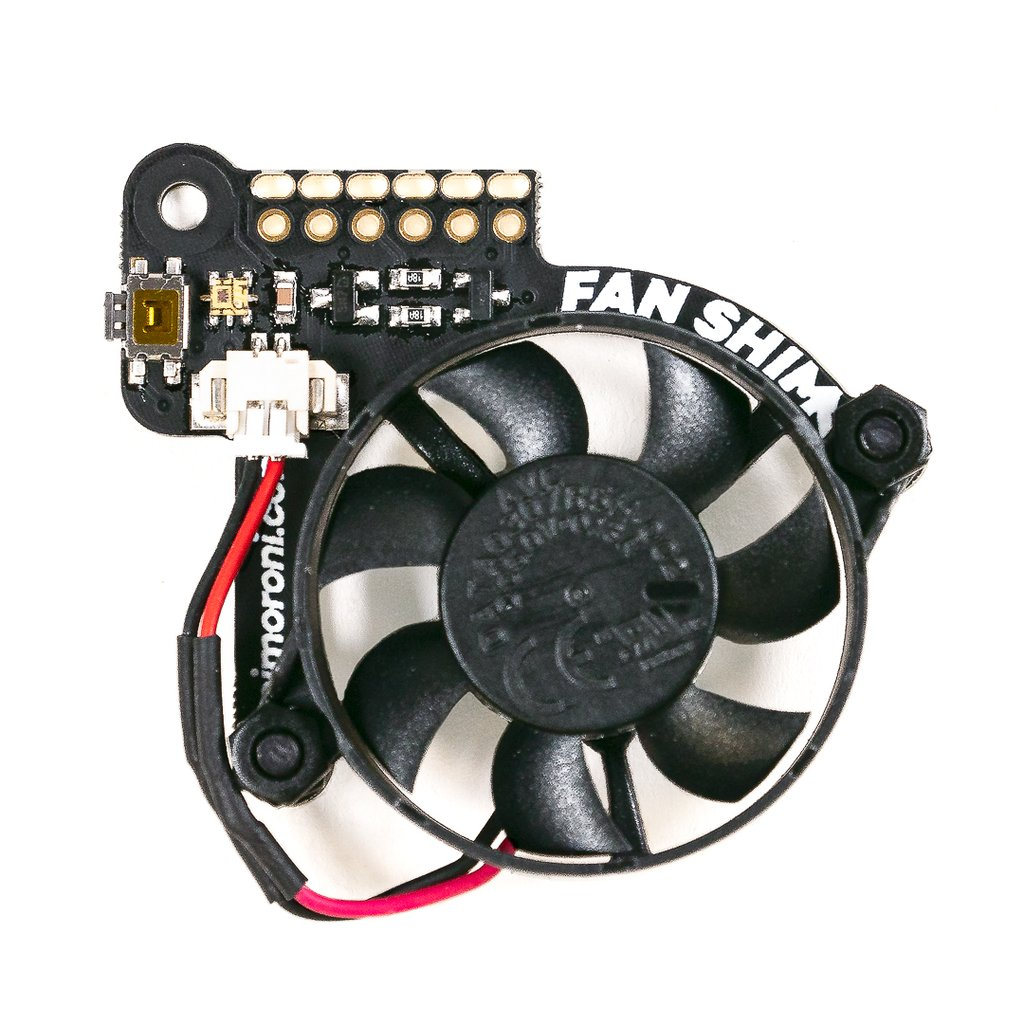
\includegraphics[width=1\linewidth]{../Figures/raspberry_pi/fan-shim.jpg}
        \vspace{0.1em}
        \caption{}
        \label{fig:raspberry_pi_shim_fan}
    \end{subfigure}
     \hspace{0.5em}
    \begin{subfigure}[b]{.25\textwidth}
        \centering
        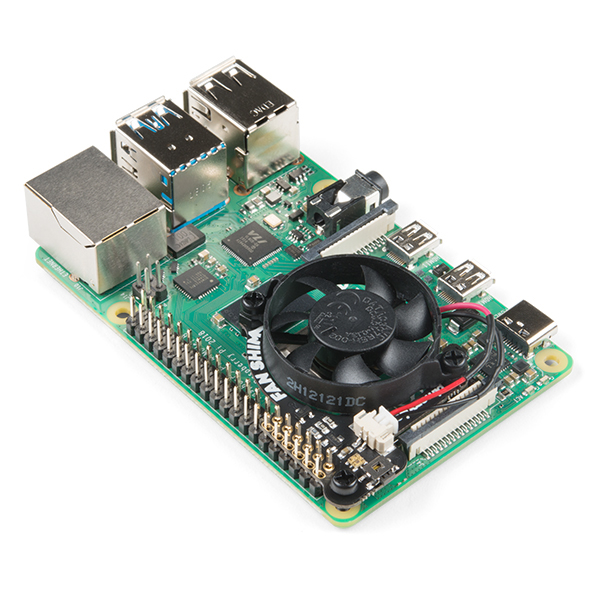
\includegraphics[width=1\linewidth]{../Figures/raspberry_pi/raspberry_pi.jpg}
          \vspace{-2.0em}
        \caption{}
        \label{fig:raspberry_pi}
    \end{subfigure}
     \hspace{-0.5em}
        \begin{subfigure}[b]{.30\textwidth}
        \centering
        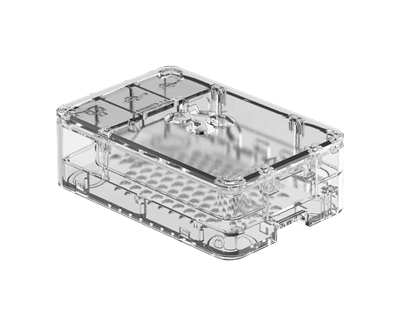
\includegraphics[width=1\linewidth]{../Figures/raspberry_pi/raspberry_pi_case.png}
         \vspace{-2.3em}
        \caption{}
        \label{fig:raspberry_pi_case}
    \end{subfigure}
            \begin{subfigure}[b]{.07\textwidth}
        \centering
        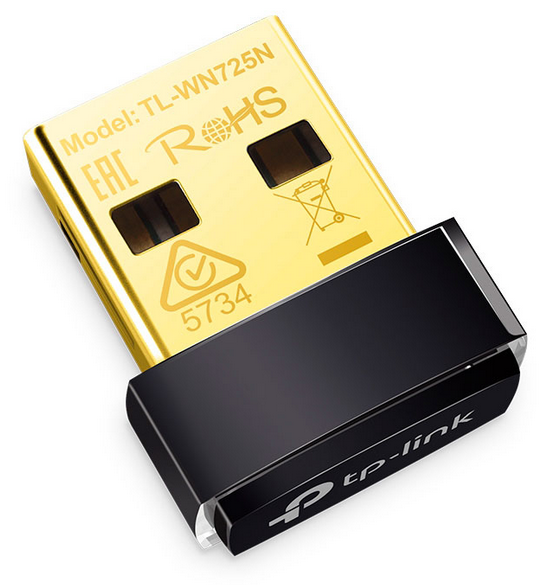
\includegraphics[width=1\linewidth]{../Figures/tpLinkac600.png}
         \vspace{1.0em}
        \caption{}
        \label{fig:tpLinkac}
    \end{subfigure}
     \hspace{-2.0em}
          \hspace{8.0em}
        \begin{subfigure}[b]{.17\textwidth}
        \centering
        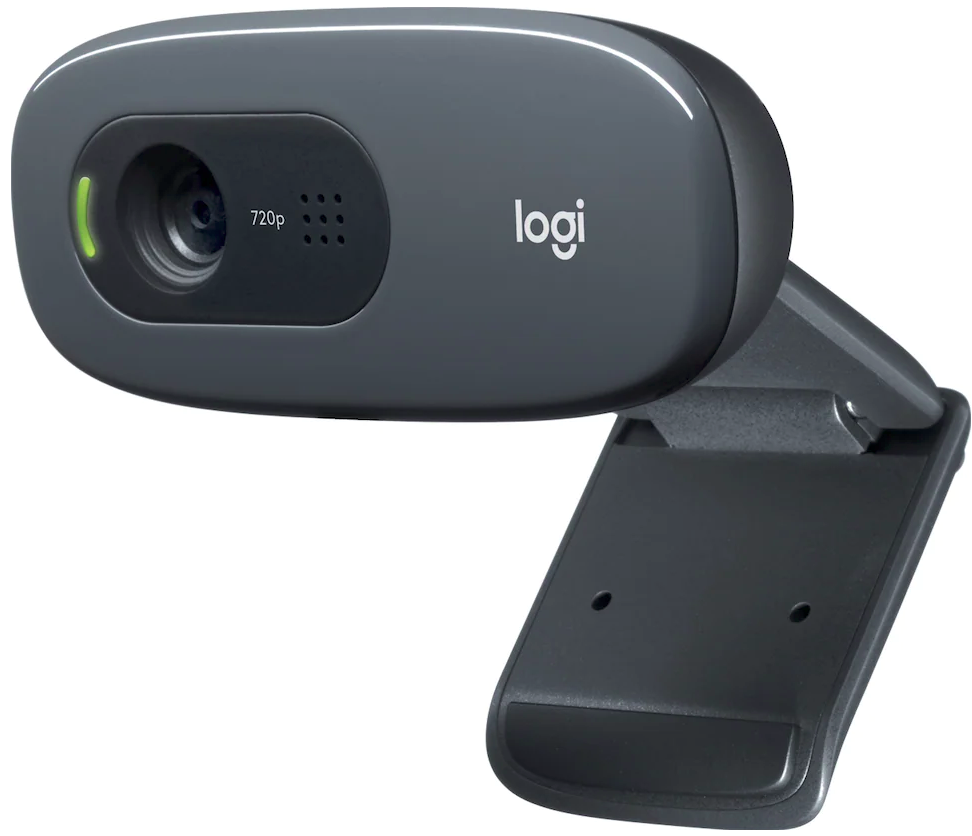
\includegraphics[width=1\linewidth]{../Figures/raspberry_pi/c270_dh_webcam.png}
         \vspace{-1.8em}
        \caption{}
        \label{fig:raspberry_pi_front_cam}
    \end{subfigure}
         \hspace{2.5em}
        \begin{subfigure}[b]{.16\textwidth}
        \centering
        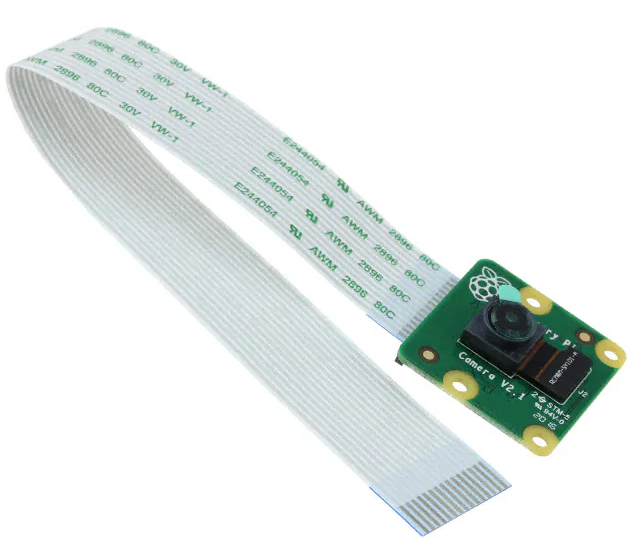
\includegraphics[width=1\linewidth]{../Figures/raspberry_pi/raspberry_pi_cam.png}
         \vspace{-1.5em}
        \caption{}
        \label{fig:raspberry_pi_bottom_cam}
    \end{subfigure}
    \caption{The \href{https://raspberrypi.dk/produkt/raspberry-pi-4-model-b-8-gb/?gclid=CjwKCAjwmv-DBhAMEiwA7xYrd2LC9iHY0AN25mCwZ8Fs49enGRBWJXCx4h8_iUrUABRWneCpaoBL1xoCoqEQAvD_BwE}{Raspberry Pi 4} can be seen in Figure \ref{fig:raspberry_pi} with the \href{https://raspberrypi.dk/produkt/blaeser-shim-til-raspberry-pi/?gclid=CjwKCAjwmv-DBhAMEiwA7xYrd5JllLUeSBohDiBjfJkpH86XFp8hRJX4kEt2lRBBwthX2DqVFSvOvRoCUykQAvD_BwE}{SHIM fan} connected. The \href{https://www.dustinhome.dk/product/5011141918/okdo-raspberry-pi-4-standard-case-clear?ssel=false&gclid=CjwKCAjwmv-DBhAMEiwA7xYrd0phkQRZwAqPH6RzFVFdcMyjZXHYr7NCCICoSREcjA1byAvG8ZpApRoCPEoQAvD_BwE}{case} for the Raspberry Pi can be seen in Figure \ref{fig:raspberry_pi_case}. The used USB WiFi adapter from \href{https://www.avxperten.dk/usb-wifi-adapter/usb-wifi-adapter-600mbps-tp-link-archer-t2u-nano.asp}{TP-Link} can be seen in Figure \ref{fig:tpLinkac}. Lastly, the \href{https://www.elgiganten.dk/product/pc-tablets/webcam/162136/logitech-c270-hd-webkamera?gclid=CjwKCAjwmv-DBhAMEiwA7xYrdzGYXgj59-xIbjHVtHUrPCTyhi44RPsqtSSi8ABd0mK8TRYZaIw8CxoC8nIQAvD_BwE&gclsrc=aw.ds}{Logitech C270 HD} and \href{https://www.proshop.dk/Mini-PC-Android-Raspberry-Pi/Raspberry-Pi-Camera-V2/2621958?utm_source=google&utm_medium=cpc&utm_campaign=searchengine&gclid=CjwKCAjwmv-DBhAMEiwA7xYrd8j1kjOx7KOcc9q1OgHUSgPDvirQwUCqQY-arqanNgdlmTPhYd3GkRoC0L8QAvD_BwE}{Raspberry Pi V2} cameras can be seen in Figures \ref{fig:raspberry_pi_front_cam} and \ref{fig:raspberry_pi_bottom_cam} respectively}
    \label{fig:raspberry_pi_hardware}
\end{figure}

\begin{figure}[H]
    \centering
    \hspace{-6.0em}
    \begin{subfigure}[b]{.4\textwidth}
        \centering
        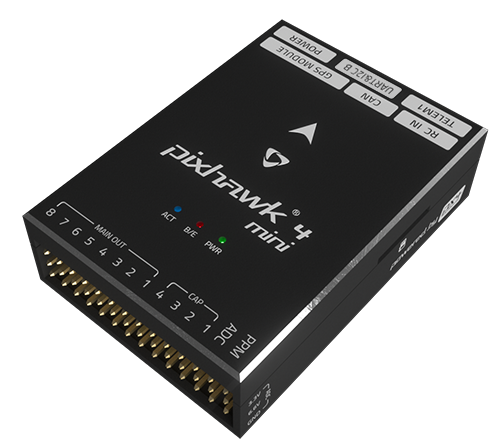
\includegraphics[height=3.5cm]{../Figures/px4_mini/px4_mini.png}
        \caption{}
        \label{fig:pixhawk_mini_four_board}
    \end{subfigure}
    %\hspace{-2.8em}
    \begin{subfigure}[b]{.33\textwidth}
        \centering
        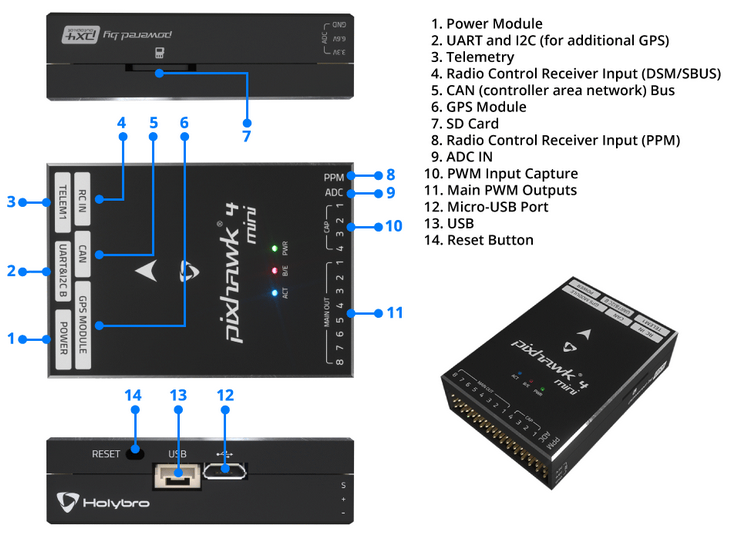
\includegraphics[height=3.5cm]{../Figures/px4_mini/px4_mini_interfaces.png}
        \caption{}
        \label{fig:pixhawk_mini_four_interfaces}
    \end{subfigure}
    \caption{Illustration of the \href{https://docs.px4.io/master/en/flight_controller/pixhawk4_mini.html}{Pixhawk 4 mini} in Figure \ref{fig:pixhawk_mini_four_board} and interface connections in Figure \ref{fig:pixhawk_mini_four_interfaces}}
    \label{fig:pixhawk_mini_four}
\end{figure}

The Pixhawk 4 mini can be seen in Figure \ref{fig:pixhawk_mini_four_board} with all interfaces in Figure \ref{fig:pixhawk_mini_four_interfaces}. The PX4 features accelerometers, gyros, a magnetometer and barometer along with a 32-bit arm cortex-m7 processer for computing. For communication, a number of serials ports (UART) are included in the PX4. For more information, a link to a detailed description of all features of the board can be seen in Figure \ref{fig:pixhawk_mini_four}. 

All connections between the user, PX4 and Raspberry Pi can be seen in Figure \ref{fig:wiring_diagram}. The green boxes indicate hardware which the user can interact with the UAV. The ground control station (GCS) is software installed in the computer from where communication between the GCS and PX4 is giving. This can be commands directly passed to the PX4 system from the GCS e.g takeoff, landing, UAV whereabouts etc. This is done from a set of transmit/receiver pairs attached to the computer by a \textit{USB connection} and the other to the PX4 using the \textit{Telem} interface (UART). In order to take command of the UAV from manual flying, the pilot can do so by using the transmitter which is connected to the PX4 using a radio receiver module connected through \textit{RCIN}. The telemetry links along with the GPS can be seen in the yellow boxes, where the GPS is attached to the GPS input of the PX4. 

To communicate directly with the Raspberry Pi, an access point can be set up from a hot-spot or wireless connection to a WiFi network. The configuration of this will be explained in Section \ref{sec:companion_computer}. This enables commands directly passed to the Raspberry Pi for controlling the UAV or video streaming of the cameras to the laptop.

The shim fan is connected to the Raspberry Pi from the GPIOs. This is because the fan can be set with a curtain speed of rotation to take into account the temperature of the CPU to act accordingly. All of the hardware directly associated with the Raspberry Pi are labeled red.  

Through the output pins of the PX4, power is regulated using electronic speed controllers (ESC) before past to the four motors connected to the propellers of the UAV. As already mentioned, the batteries are connected separately to the PX4 and Raspberry Pi through power converters from where constant and stable voltage and current are giving to the two units.   

\begin{figure}[H]
    \centering
     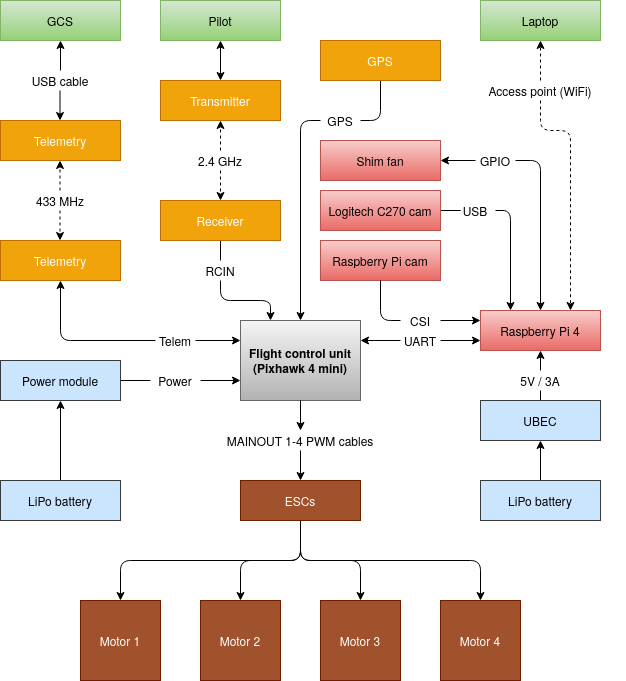
\includegraphics[height=11.0cm]{../Figures/power_system/power_system.png}
    \caption{The wiring diagram which illustrates the setup of all connections between hardware. Green boxes defines user interactions with the PX4 and Raspberry Pi, yellow boxes communication modules and GPS, blue boxes the batteries and converters, brown boxes motors and regulators, red boxes Raspberry Pi and associated hardware and lastly the PX4 flight controller labeled gray. Solid and dotted lines defines wire and wireless connection respectively}
    \label{fig:wiring_diagram}
\end{figure}

The final configuration of the QAV250 Quadcopter can be seen in Figure \ref{fig:drone_one} and \ref{fig:drone_two}. Here a set of feet is attached to the UAV to make room for the Raspberry Pi, which is attached at the bottom of the UAV. The GPS module has been placed at a higher position compared to the original design in order for better data transmission. Because the propellers of the UAV are near the flight controller, cables have been set close to the center of the UAV in order to avoid collisions. The web came case of the Logitech C270 HD camera has been removed to fit the UAV which is placed at the front of the UAV which can be seen in Figure \ref{fig:drone_front}. Moreover, the USB cable of the Logitech C270 HD has been shortened and re-soldered to fit in configuration of the UAV which may be noticed by the tight ordering of the cables in Figure \ref{fig:drone_close_one} and \ref{fig:drone_close_two}.    

\begin{figure}[H]
    \centering
    \begin{subfigure}[b]{.33\textwidth}
        \centering
        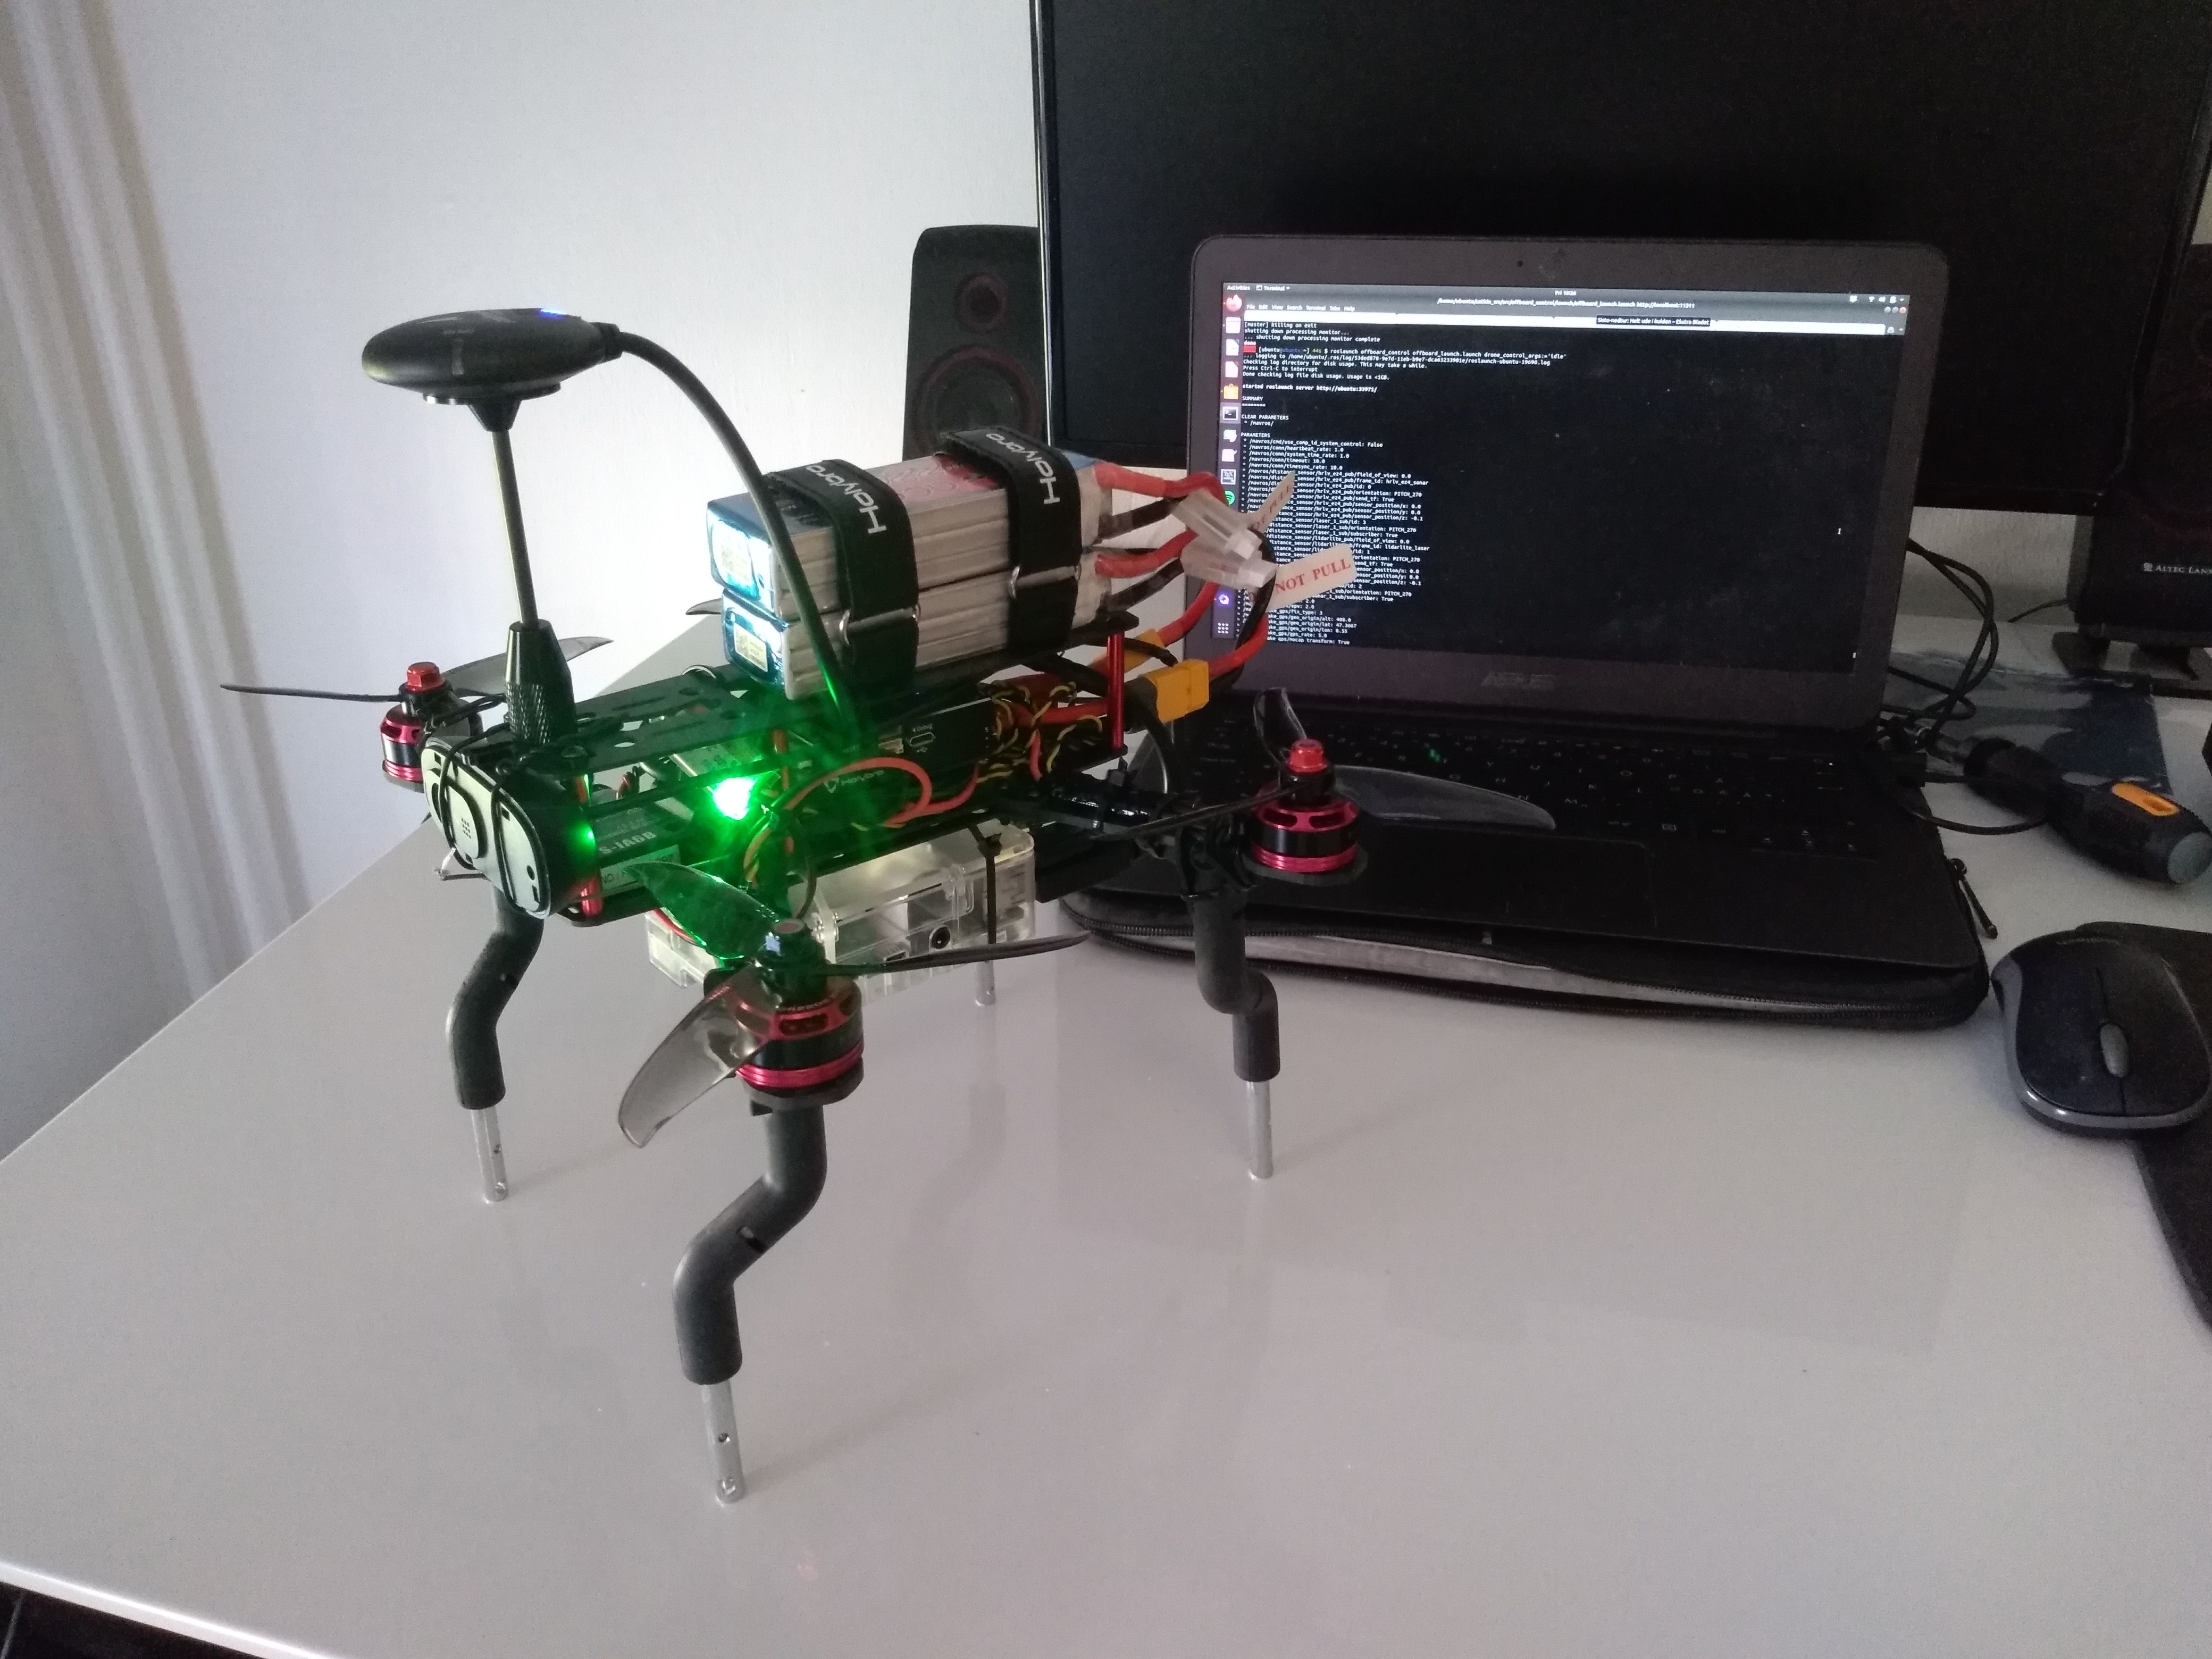
\includegraphics[height=3.6cm]{../Figures/drone/drone_front.jpg}
        \caption{}
        \label{fig:drone_front}
    \end{subfigure}
    \begin{subfigure}[b]{.33\textwidth}
        \centering
        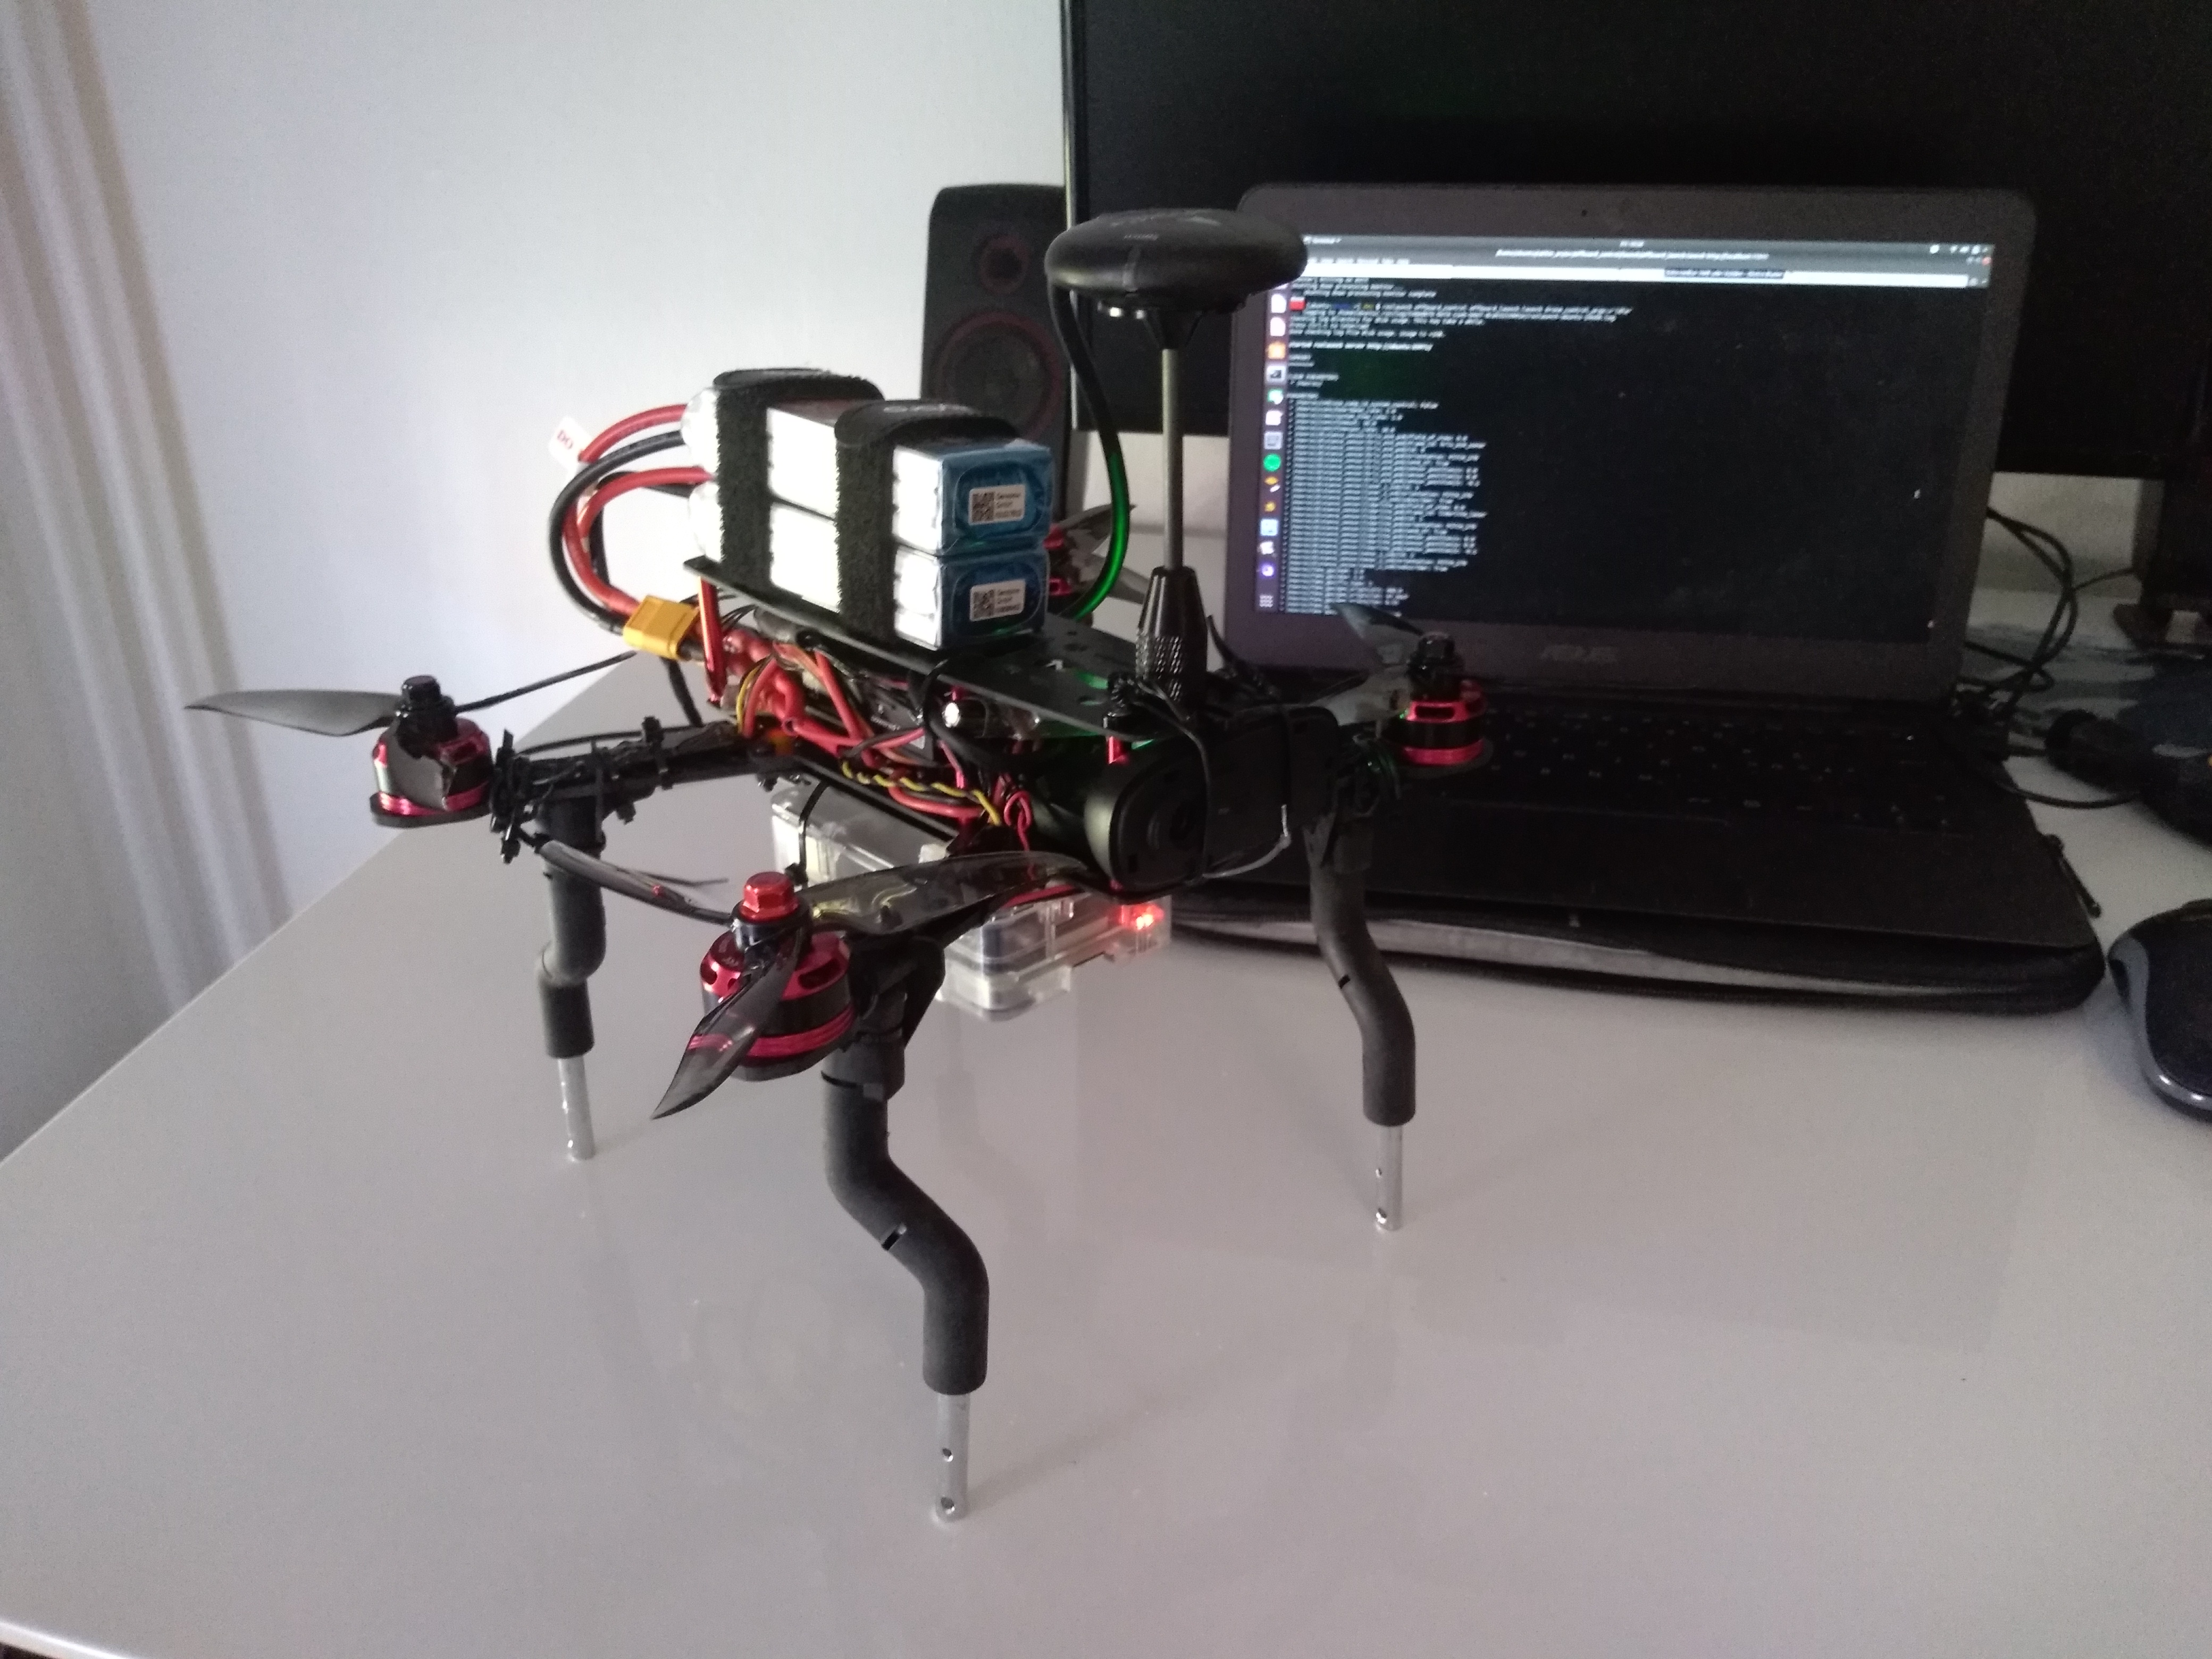
\includegraphics[height=3.6cm]{../Figures/drone/drone_front2.jpg}
        \caption{}
        \label{fig:drone_bottom_zoom}
    \end{subfigure}
    \caption{Illustration of the final updated design of the QAV250 Quadcopter. As it can be seen in Figure \ref{fig:drone_front}, a landing set has been attached to the UAV to make room for the Raspberry Pi}
    \label{fig:drone_one}
\end{figure}

\begin{figure}[H]
    \centering
    \begin{subfigure}[b]{.20\textwidth}
        \centering
        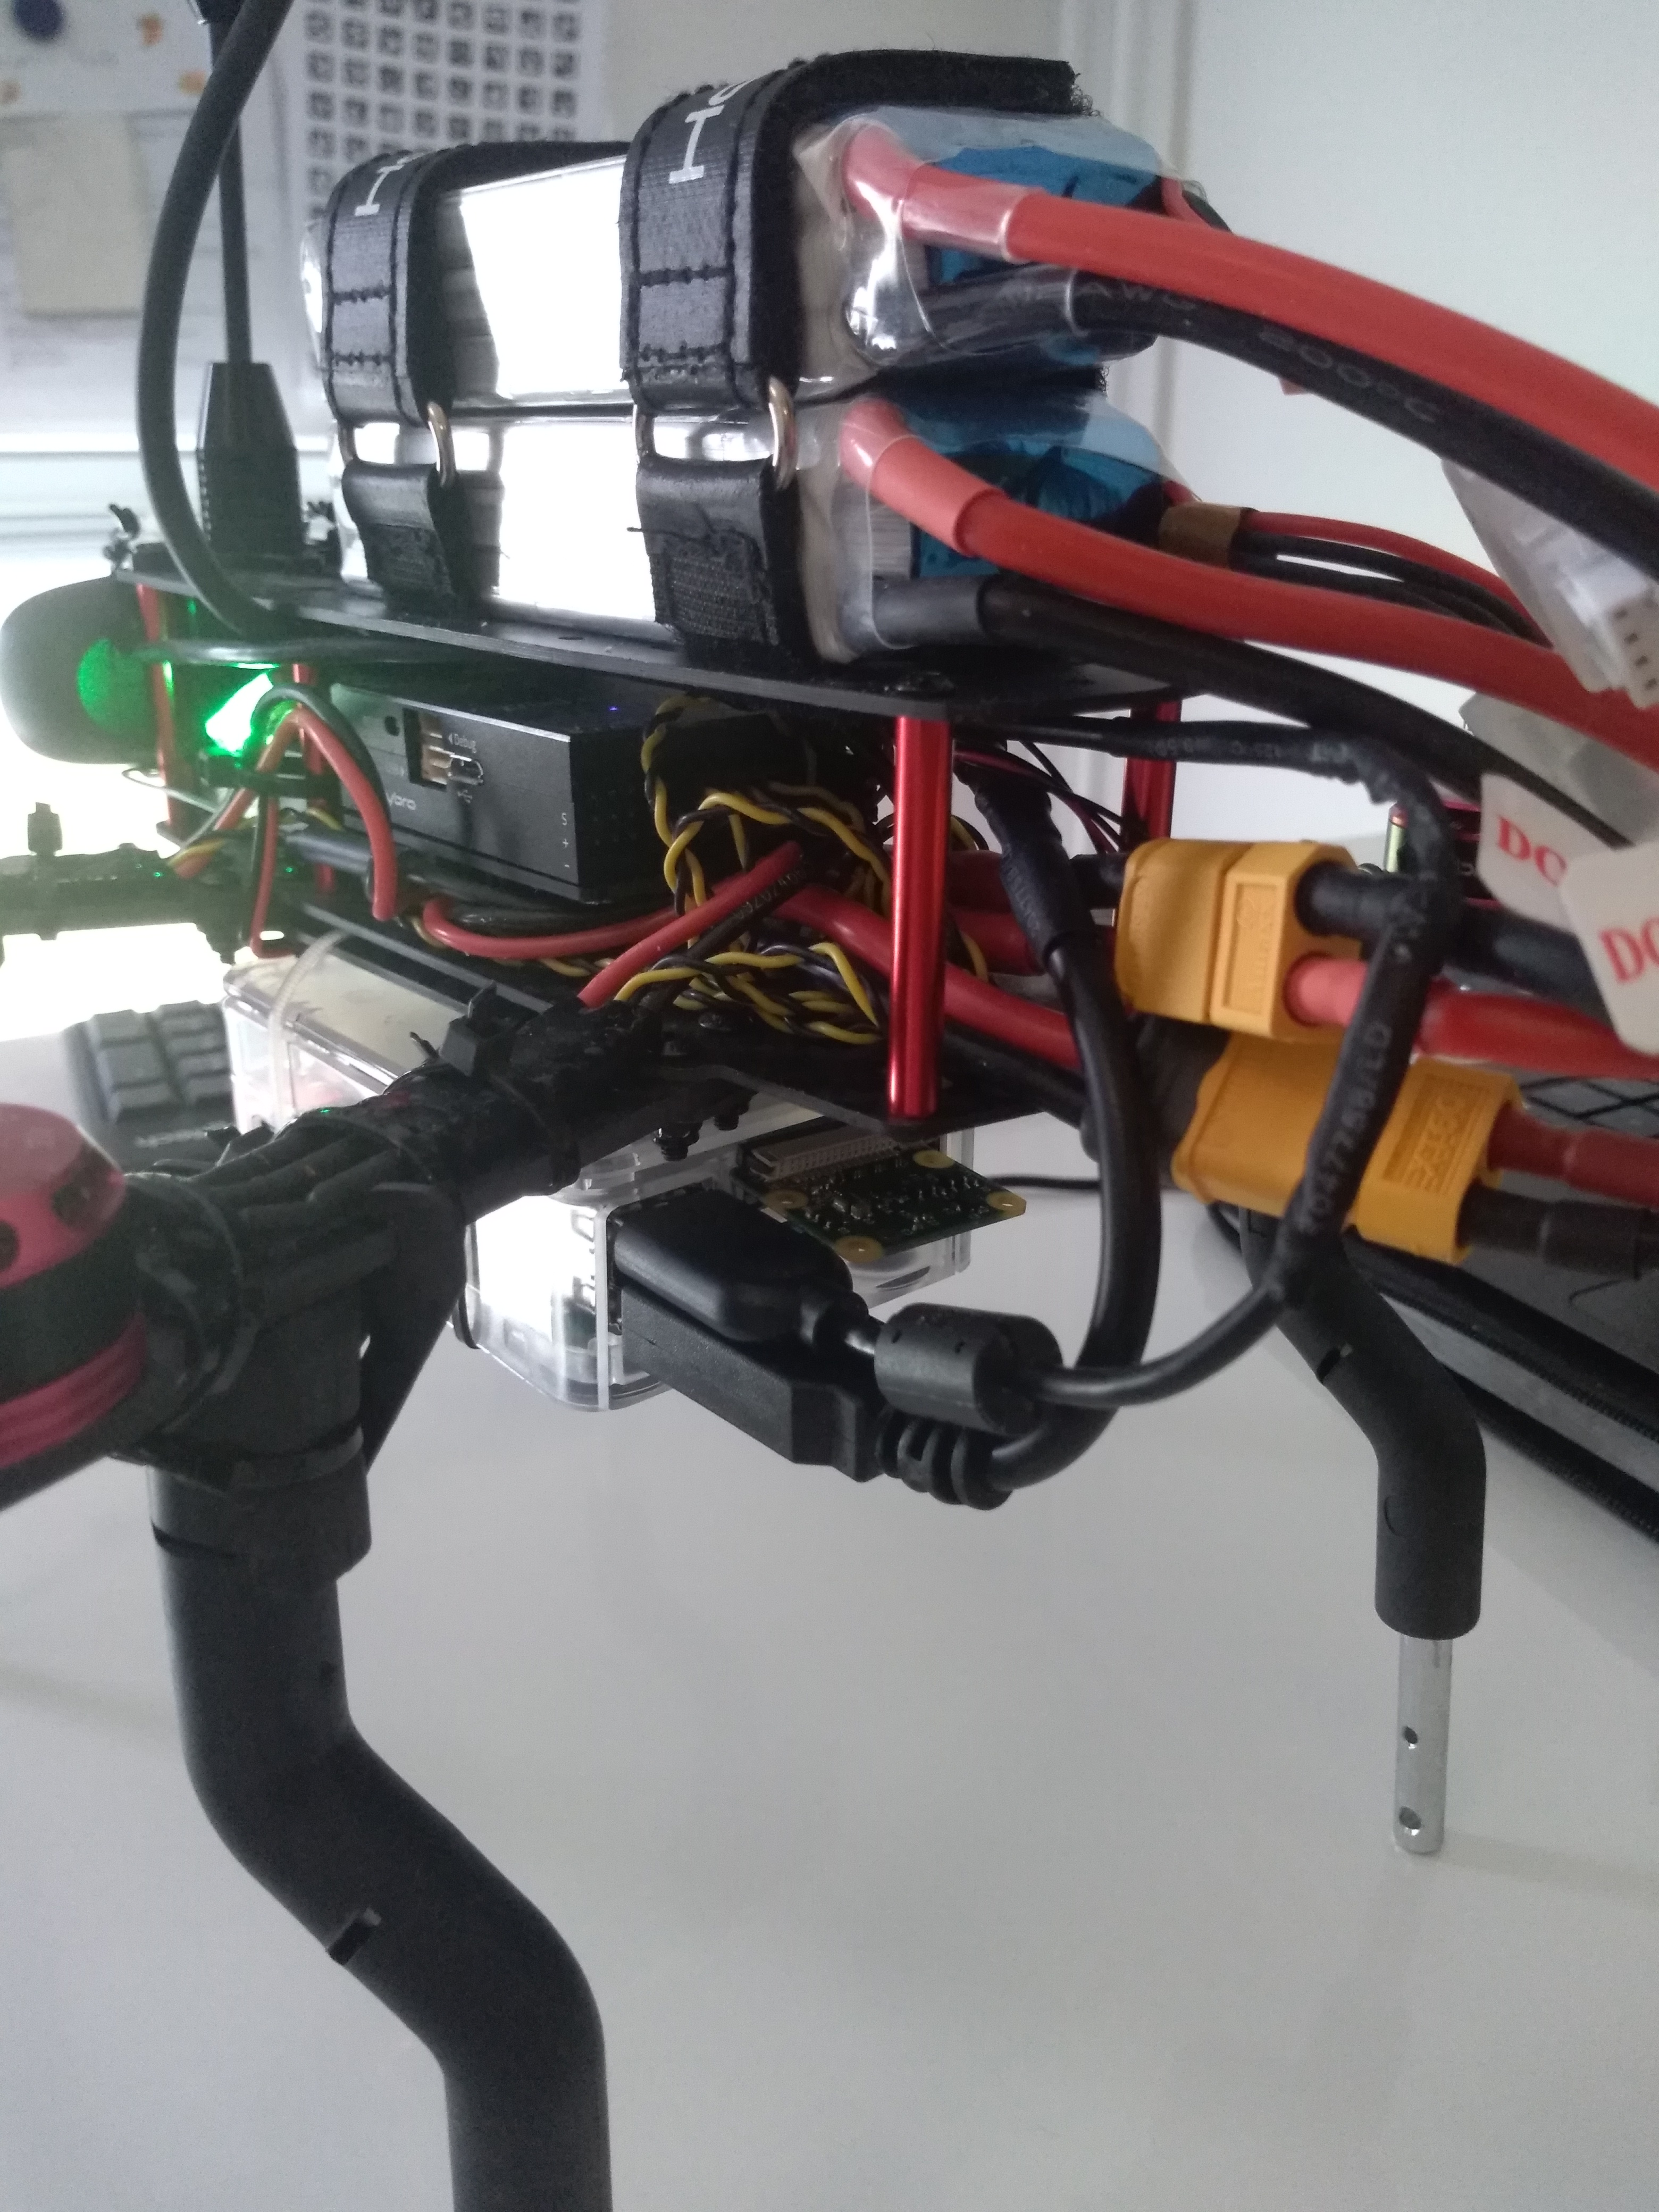
\includegraphics[height=3.6cm]{../Figures/drone/drone_close1.jpg}
        \caption{}
        \label{fig:drone_close_one}
    \end{subfigure}
    \begin{subfigure}[b]{.20\textwidth}
        \centering
        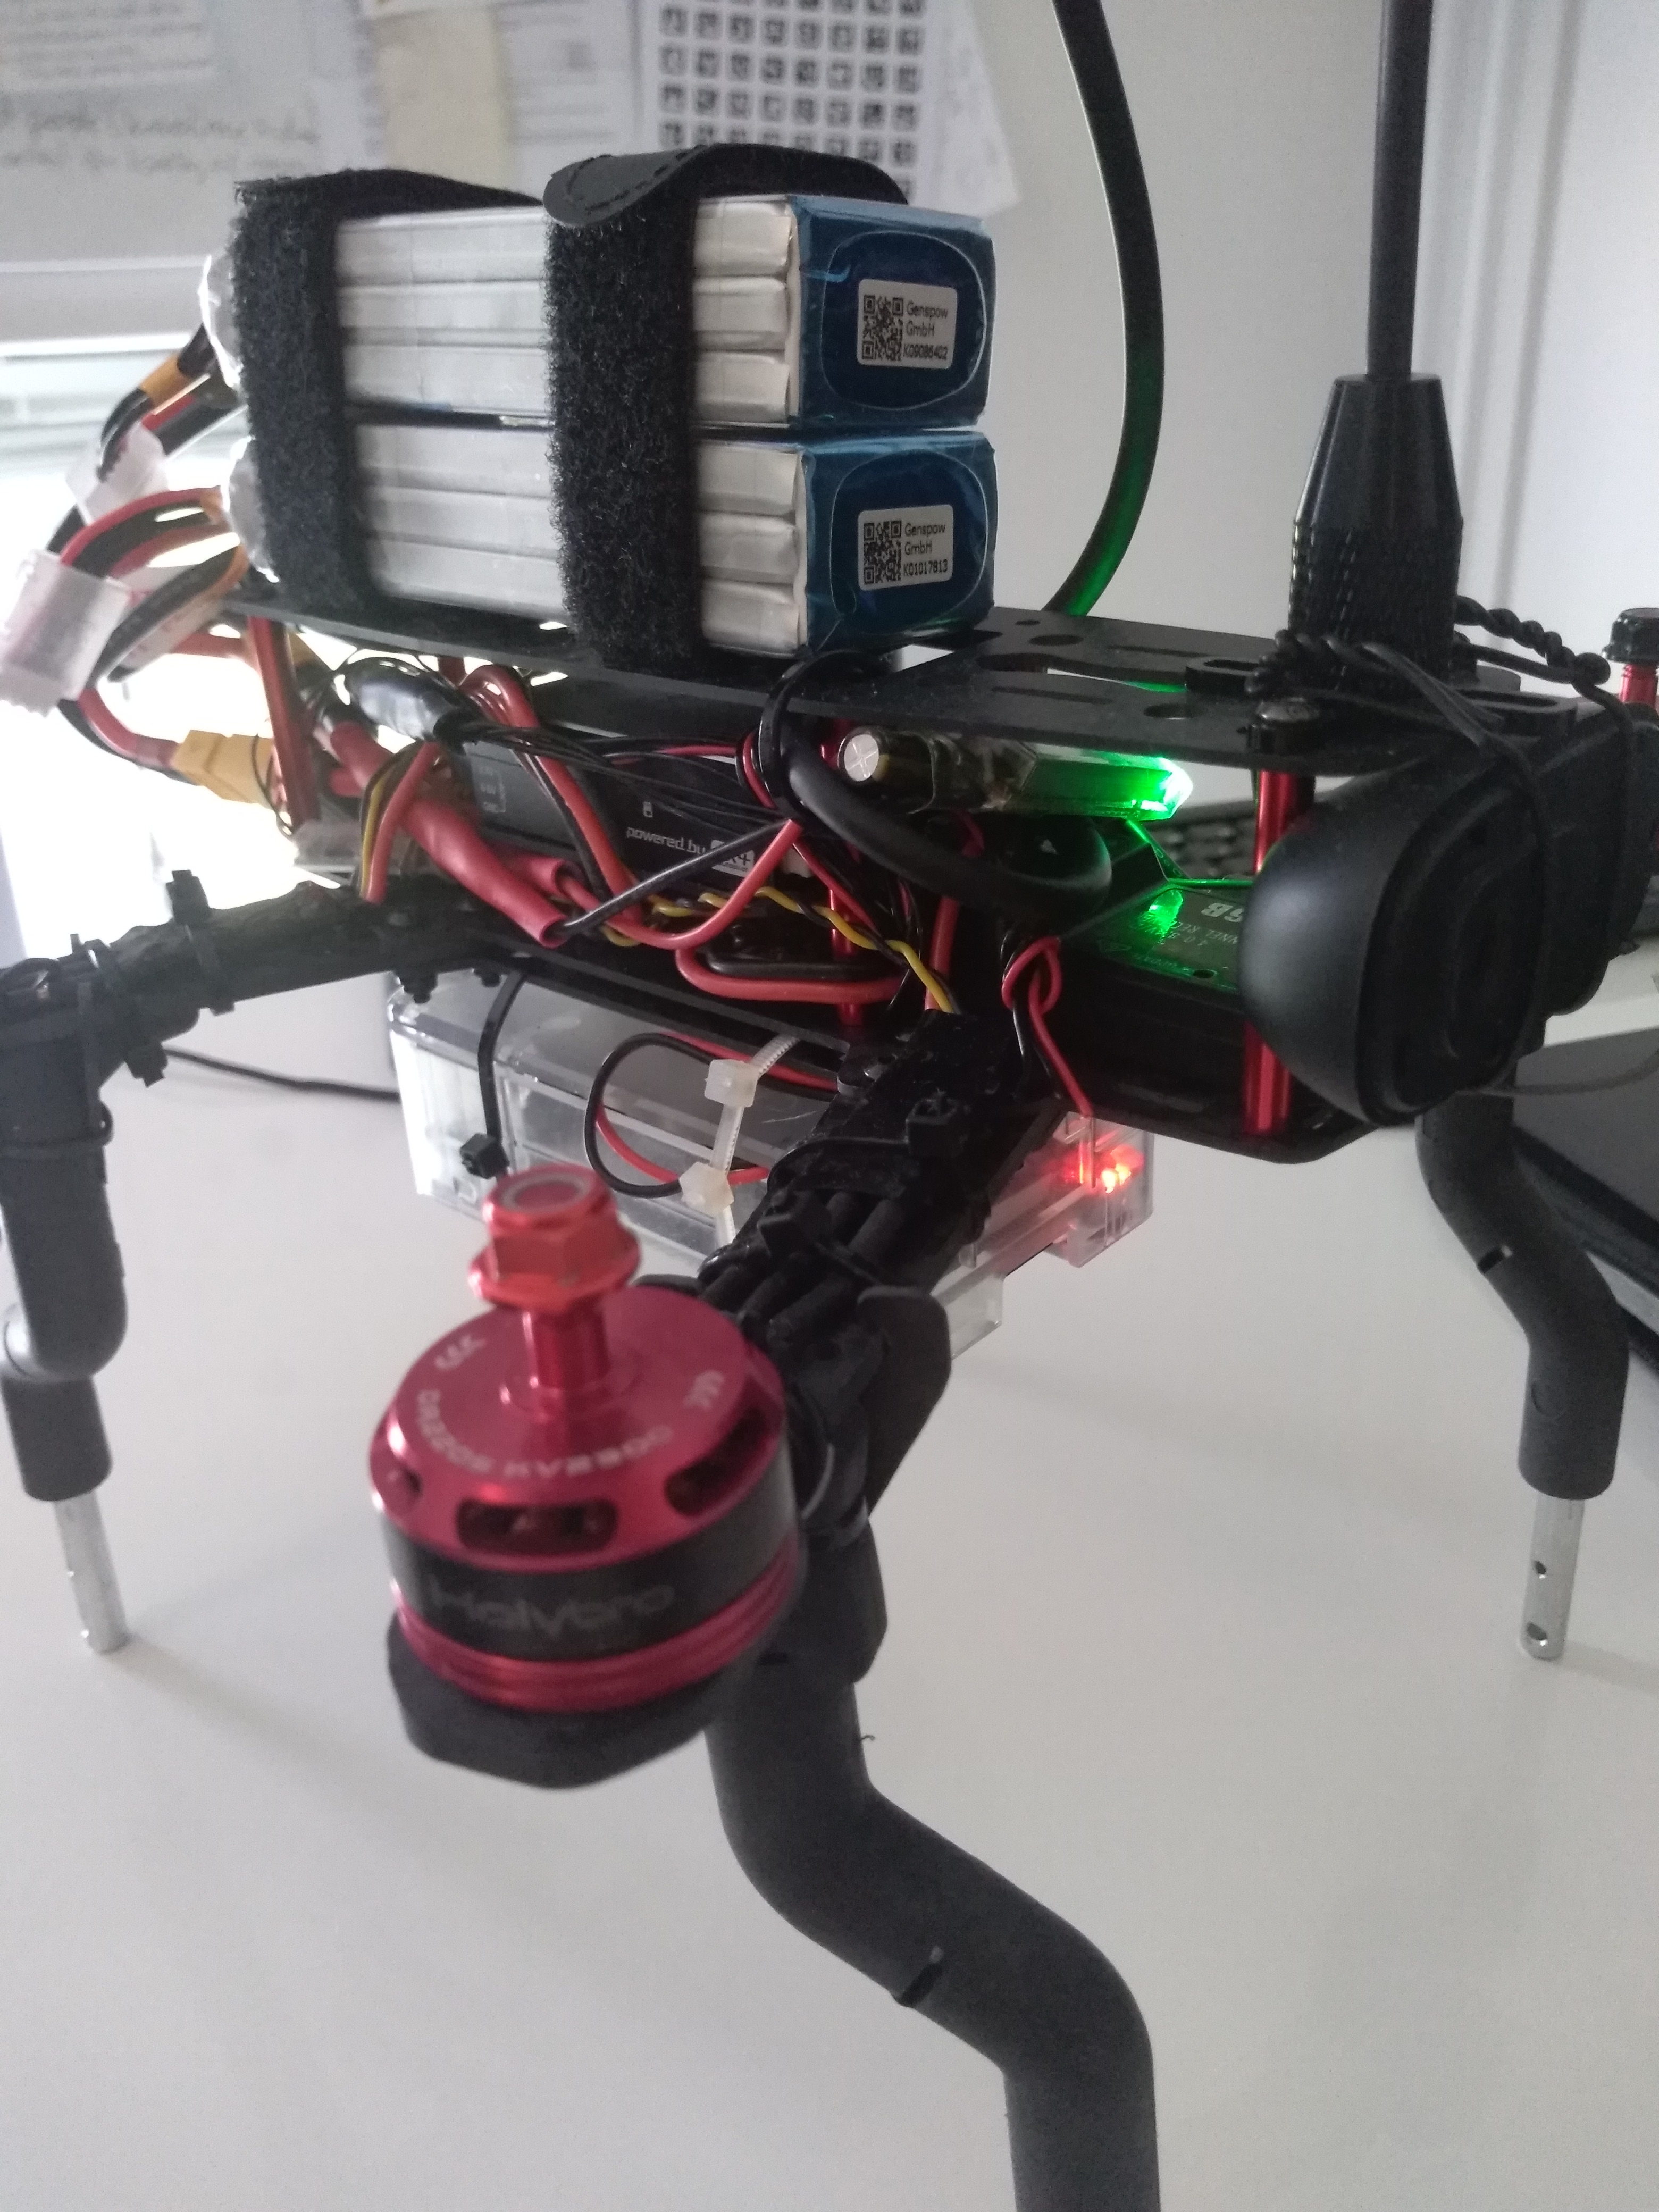
\includegraphics[height=3.6cm]{../Figures/drone/drone_close2.jpg}
        \caption{}
        \label{fig:drone_close_two}
    \end{subfigure}
    \begin{subfigure}[b]{.20\textwidth}
        \centering
        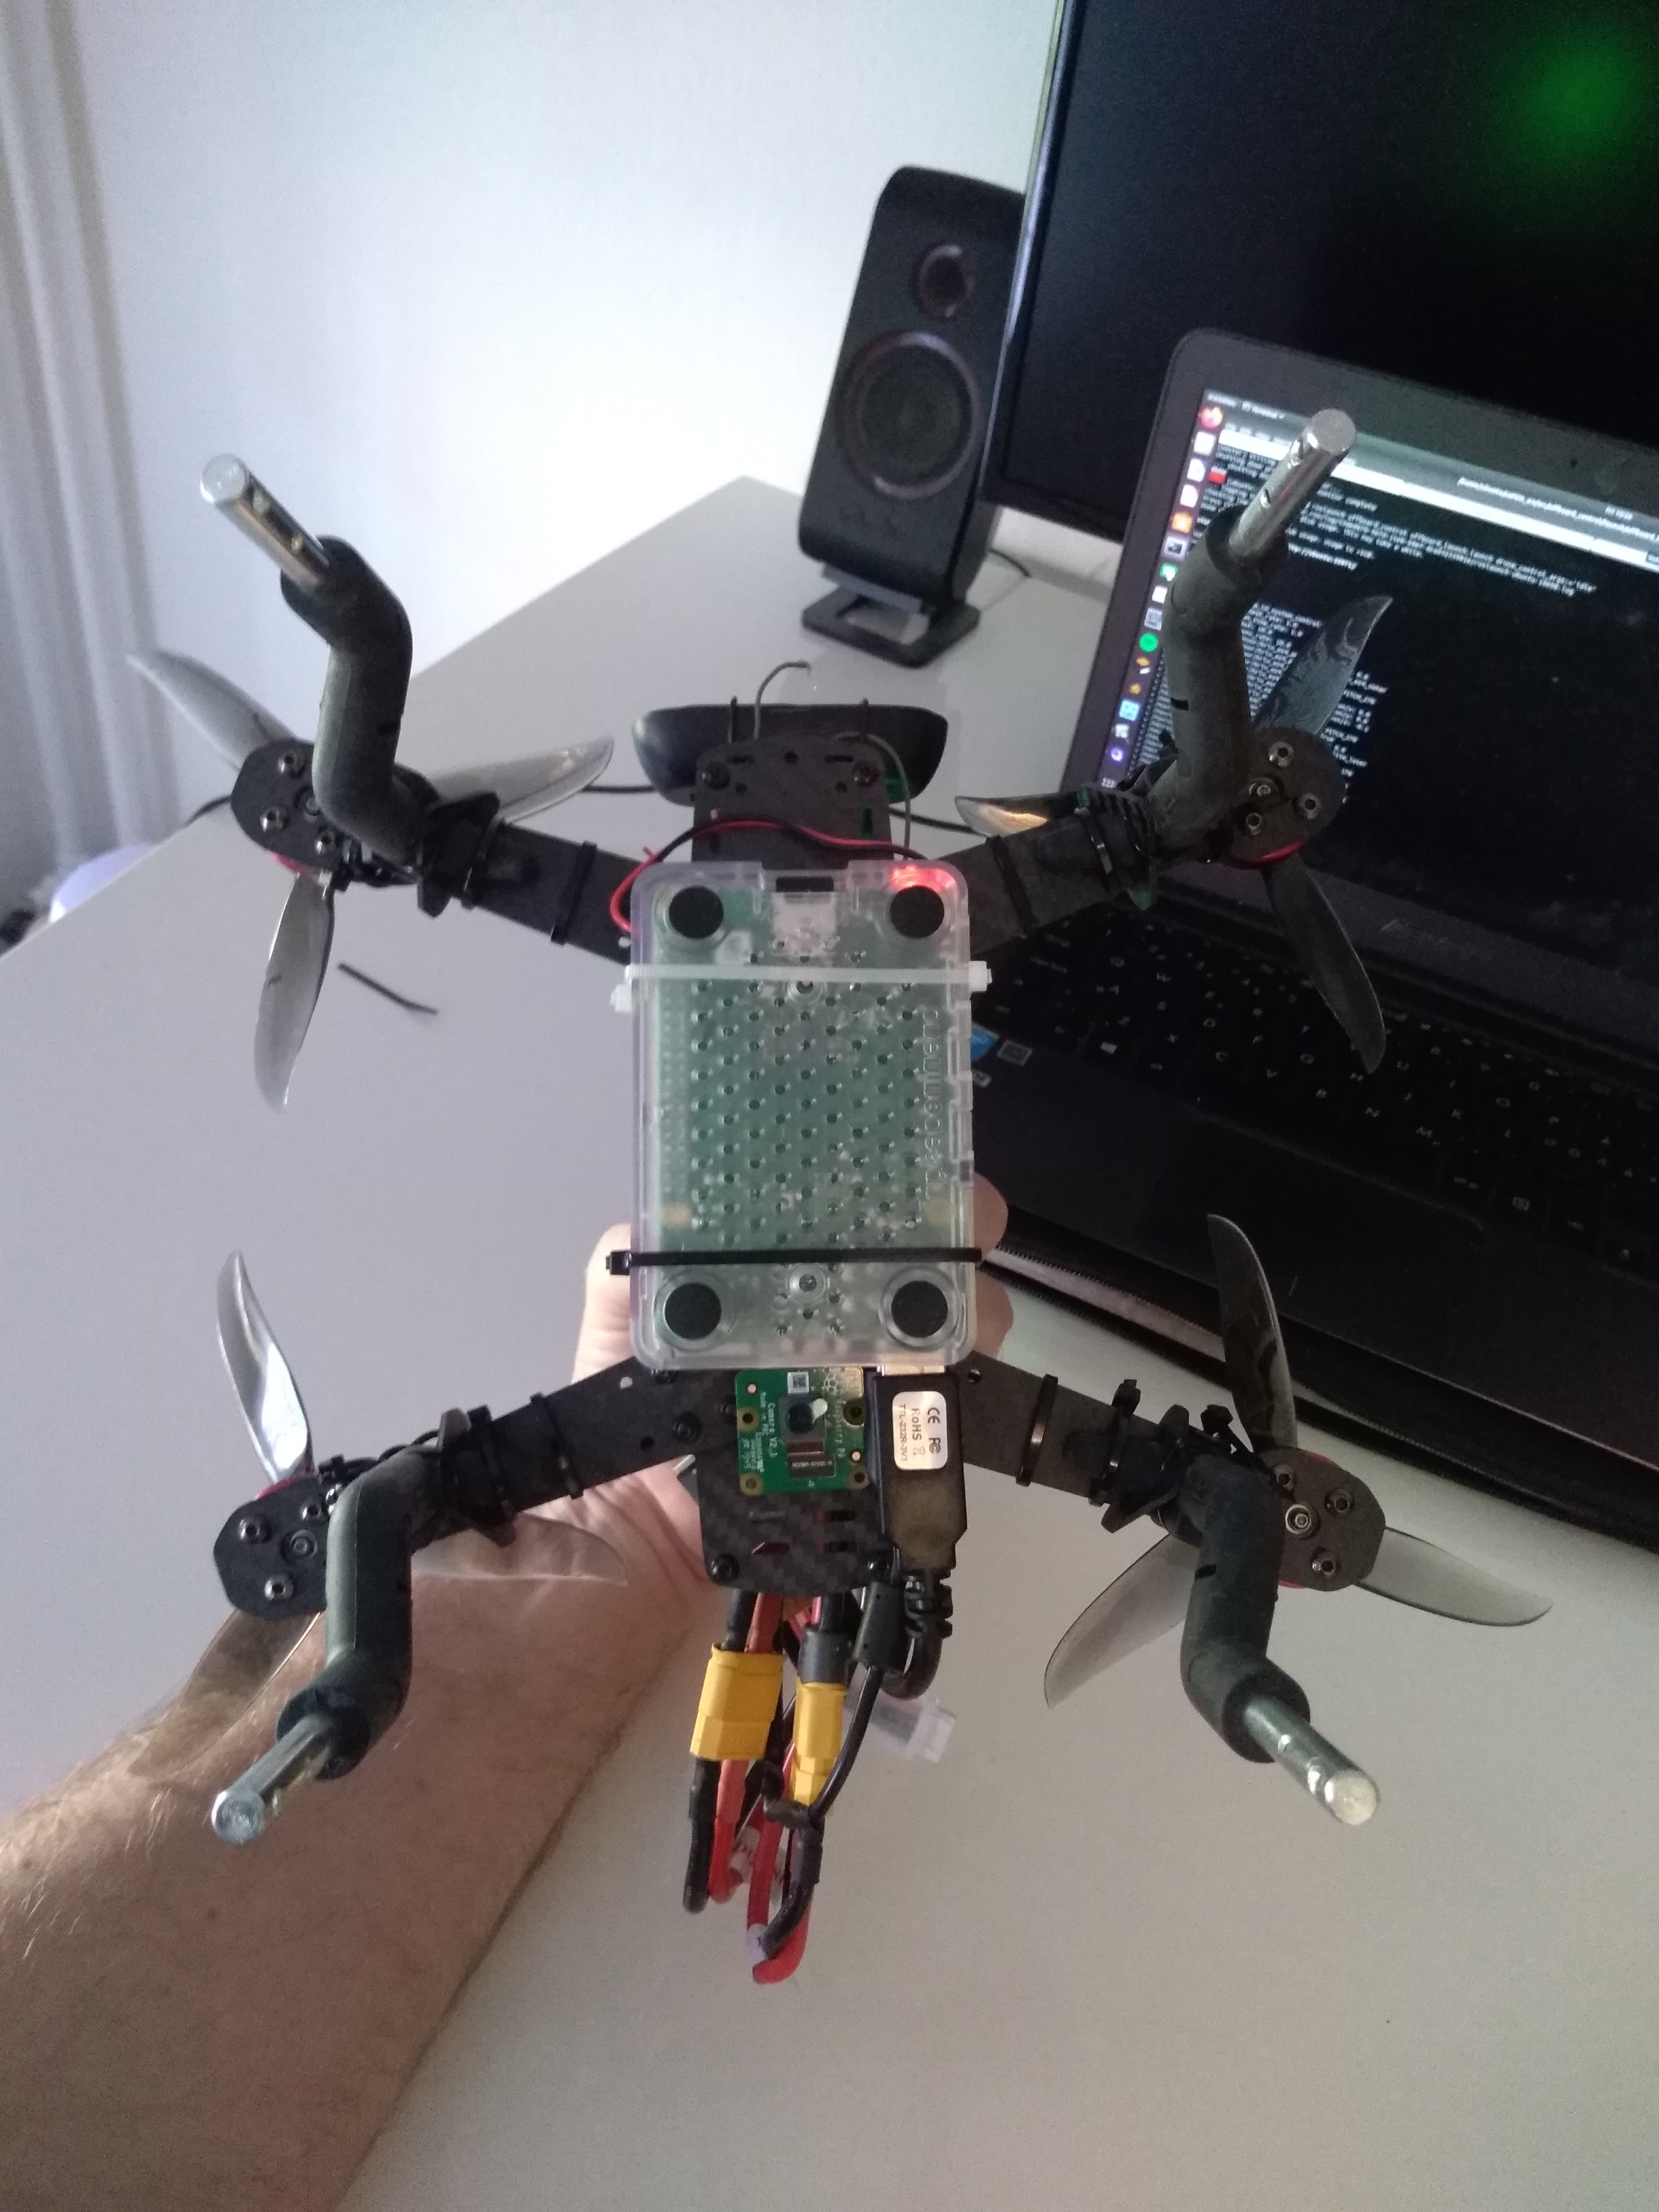
\includegraphics[height=3.6cm]{../Figures/drone/drone_bottom.jpg}
        \caption{}
        \label{fig:drone_bottom}
    \end{subfigure}
    \begin{subfigure}[b]{.20\textwidth}
        \centering
        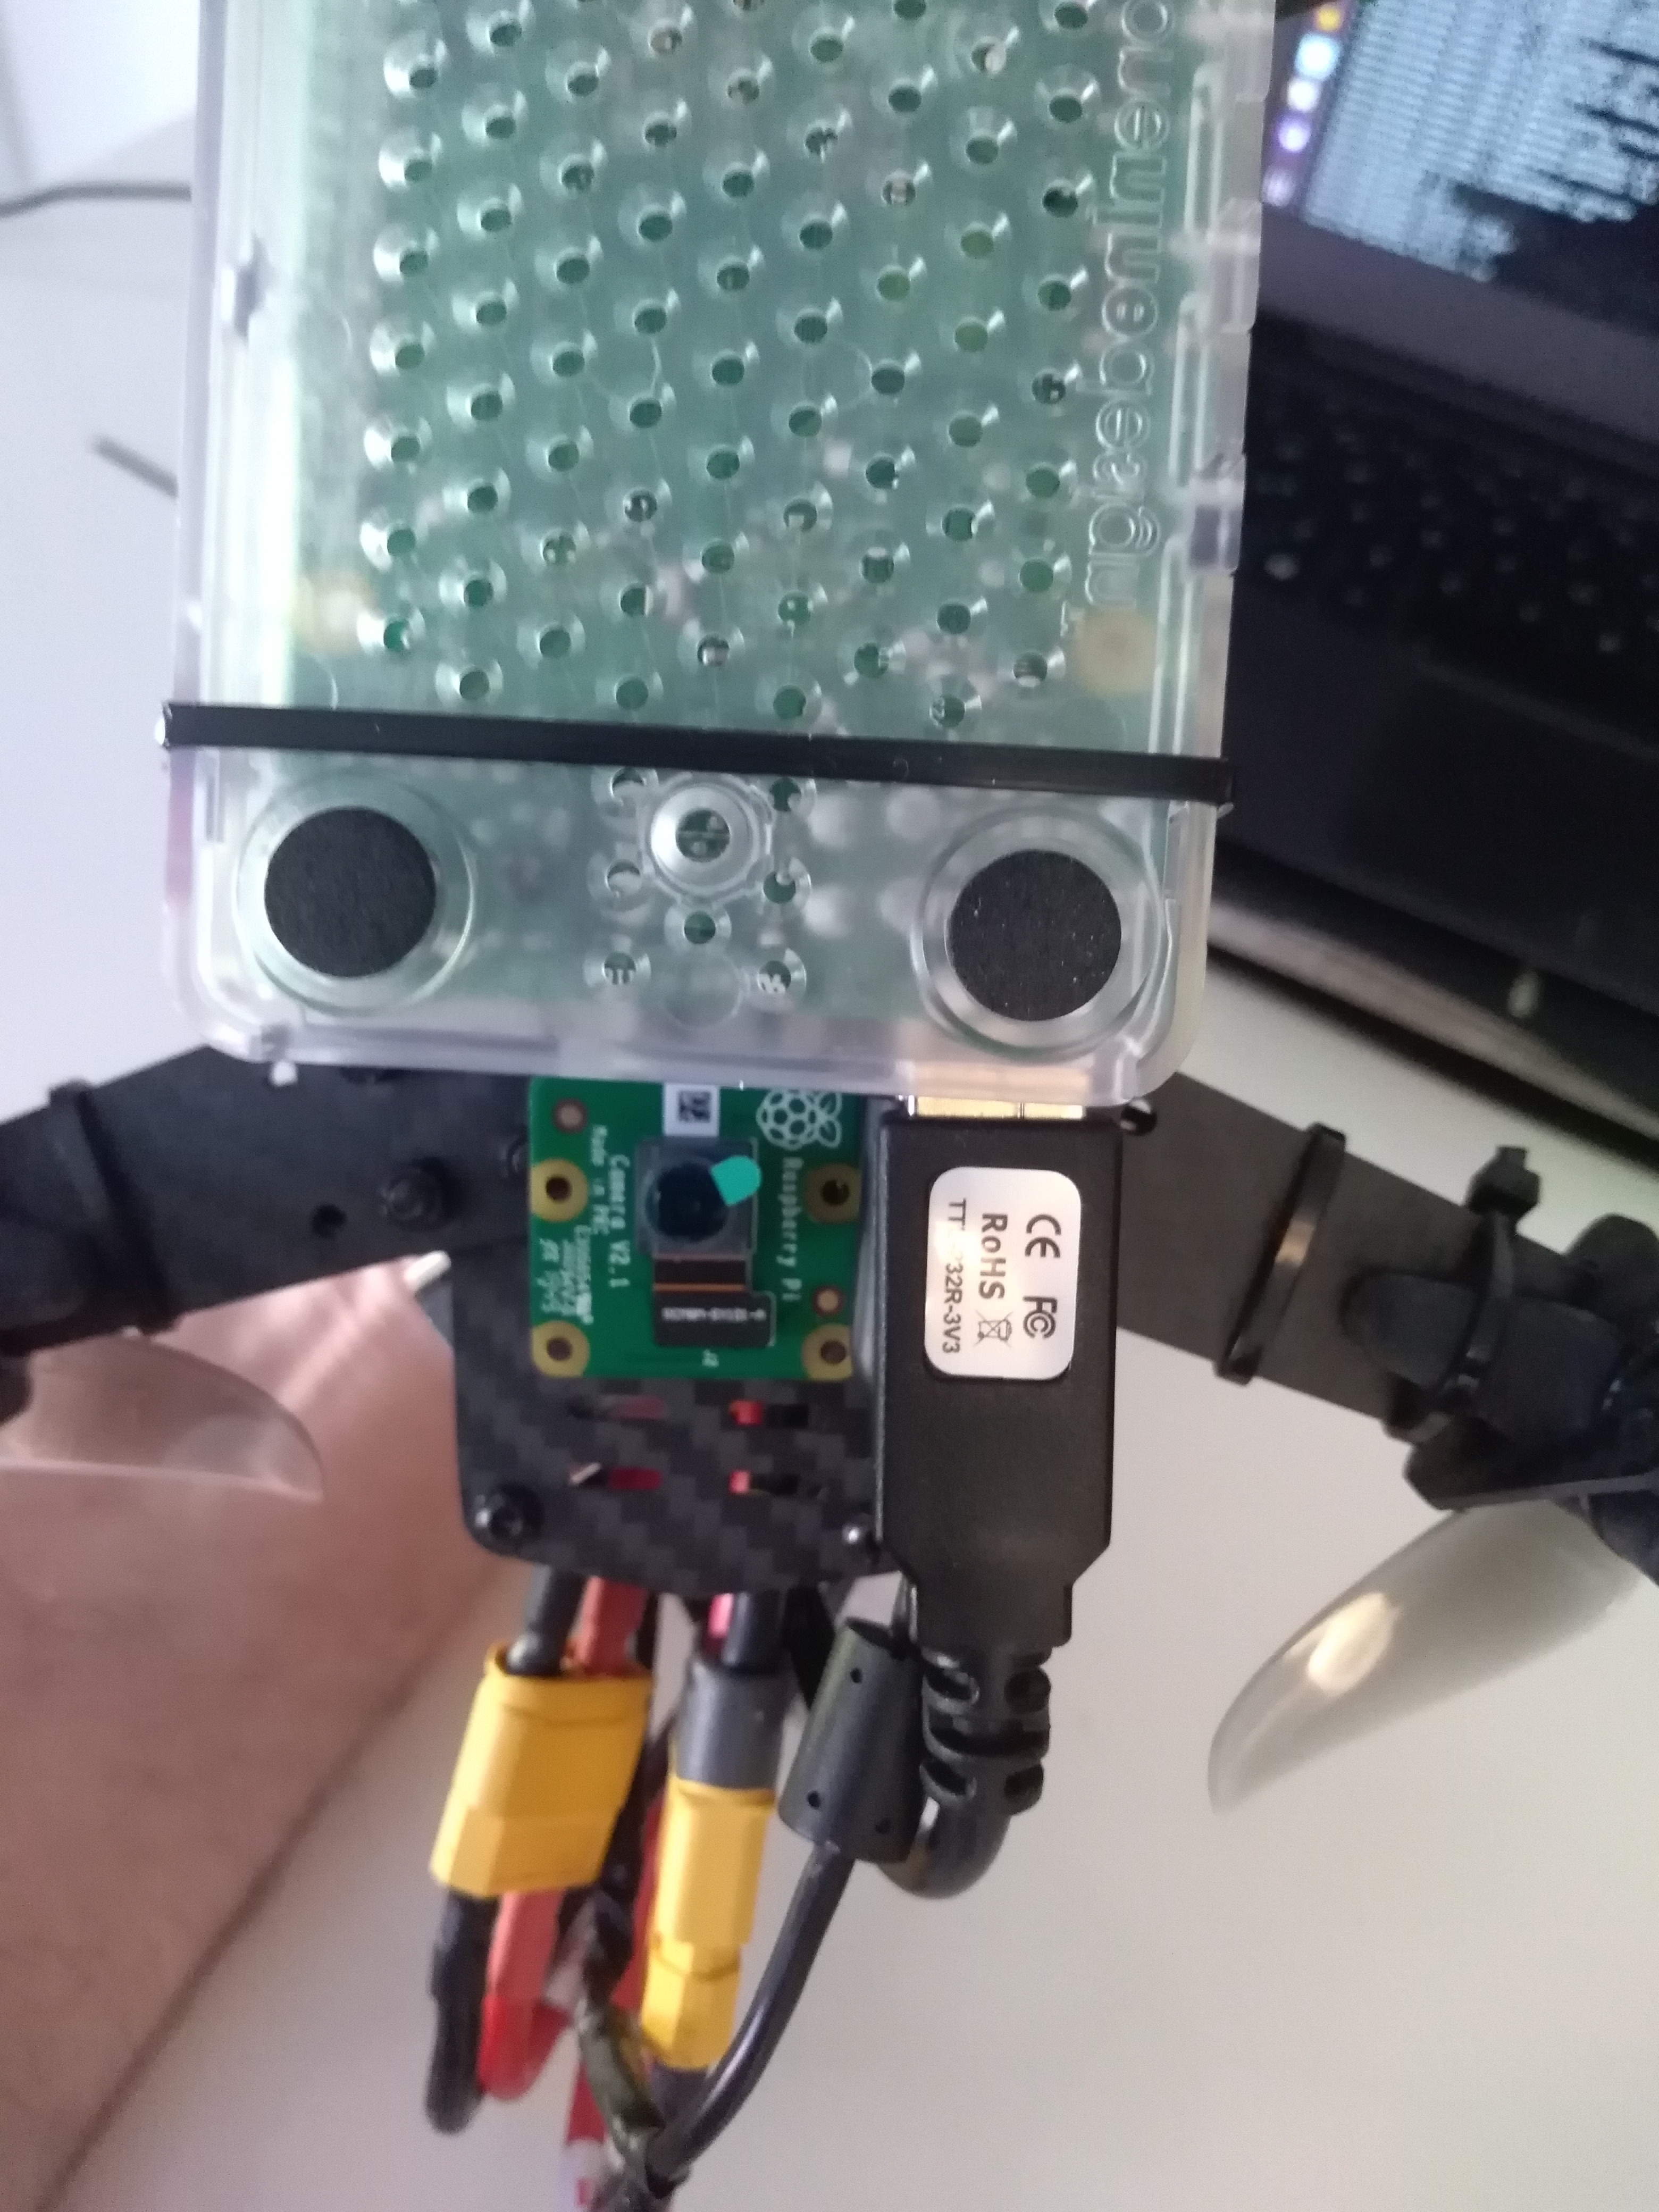
\includegraphics[height=3.6cm]{../Figures/drone/drone_bottom_zoom.jpg}
        \caption{}
        \label{fig:drone_bottom_zoom}
    \end{subfigure}
    \caption{Illustration of the final updated design of the QAV250 Quadcopter. In Figure \ref{fig:drone_bottom_zoom}, the Raspberry Pi camera is seen to pointing straight down which is accomplished by using the Raspberry case}
    \label{fig:drone_two}
\end{figure}

\subsection{Bill of materials}
\label{sec:bill_of_materials}

The materials used in this configuration can be seen in Table \ref{tab:bill_of_materials} where products, price and supplier is mentioned. It may be noticed that the overall price of the kit is approximately 4.502,14 DKK which is mostly due to the expensive items like the drone kit and Raspberry Pi 4.   

\newcommand{\done}{\cellcolor{teal}done}  %{0.9}
\newcommand{\hcyan}[1]{{\color{teal} #1}}

\begin{table}[H]
\centering
\caption{List of products with price for the materials used}
\label{tab:bill_of_materials}
\begin{tabular}{lccr}
\toprule
Products & Supplier & Amount & Price\\
\midrule

Drone (\textit{Drone and communication}) \\
\phantom{ZZ} HolyBro QAV250 + Pixhawk4-Mini & banggood.com & 1 & 2.037,73 DKK\\
\phantom{ZZ} FlySky-FS-i6-2.4G-6CH & banggood.com & 1 & 352,76 DKK \\

Batteries (\textit{Batteries and related materials}) & \\
\phantom{ZZ} Gens ace LiPo 11.1 V 2200 mAh Cell: 3 45 C XT60 & conradelektronik.dk & 2 & 249,00 DKK \\
\phantom{ZZ} KINGKONG 5V 3A Switching Power UBEC & hobbyking.com & 1 & 23,65 DKK \\
\phantom{ZZ} SKYRC e430 charger 3 A LiPo, LiFePO & banggood.com & 1 & 209,00 DKK \\
\phantom{ZZ} EXTRON Modellbau LiPo safety-bag 1 Set & cdon.dk & 1 & 259,00 DKK \\

Raspberry pi (\textit{Raspberry Pi and related materials}) & \\
\phantom{ZZ} Raspberry Pi 4 model B - 8GB & raspberrypi.dk & 1 & 669,00 DKK \\
\phantom{ZZ} Fan SHIM for Raspberry Pi & raspberrypi.dk & 1 & 99,00 DKK \\
\phantom{ZZ} Okdo Raspberry Pi 4 Standard Case Clear & dustinhome.dk & 1 & 55,00 DKK \\
\phantom{ZZ} Logitech C270 HD camera & elgiganten.dk & 1 & 249,00 DKK \\
\phantom{ZZ} Raspberry Pi Camera V2 & proshop.dk & 1 & 299,00 DKK \\
\phantom{ZZ} USB WiFi adapter & avxperten.dk & 1 & 149,00 DKK \\

\textsc{Overall product price} & & & \textbf{4.651,14 DKK} \\

\bottomrule                
\end{tabular}
\end{table}


\end{document}